
\clearpage





%...........................................................
%
% Comparison of Run 1-7c data with sensitivity
%
%...........................................................

\subsection {Comparison of $\delta_{CP}$ vs mass hierarchy Run 1-7c result with sensitivity}
\label{sec:comparison_data_sensi_dcp_run17c}

In order to understand better the output of the Run 1-7c data fit, the result 
has been compared with the expected sensitivity obtained by performing 10k toy experiments
for different true values of $\delta_{CP}$ and mass hierarchy.
The same procedure as for Run 1-7b, shown in \cref{sec:comparison_data_sensi_dcp_run17b}, is used.

\subsubsection {$\delta_{CP} = -\pi/2$ - normal hierarchy}
\label{sec:dcp_mpiover2_nh_run17c}

In \cref{fig:brazilian_mpiover2_run17c} the Run 1-7c data result for $\delta_{CP}$ vs mass hierarchy 
is compared to the expected mean $\Delta \chi^2$ ($<\Delta \chi^2>$)
distribution as well as the $1\sigma$ and $2\sigma$ 
uncertainties on the $\Delta \chi^2$ distributions
corresponding to $\delta_{CP}=-\pi/2$ and normal hierarchy.

%The sensitivity plot was obtained as following:
%\begin{itemize}
%
%\item 10k toy experiments were performed for a certain true point,
%	in this case $\delta_{CP} = -\pi/2$ and normal hierarchy,
%	and the full $\chi^2_{toy}$ distribution was computed as a function of
%	$\delta_{CP}$ and mass hierarchy, as described in \cref{sec:marginalization};
%	
%%	For each toy experiment a $\Delta \chi^2$ distribution analogue to what shown,
%%	for example, in \cref{fig:validation_sensi_dcp_run17c_a} is obtained;	
%%\item for each bin of $\delta_{CP}$ and mass hierarchy a histogram was filled with the $\Delta \chi^2$ 
%%	values of each toy experiment, corresponding to that bin of $\delta_{CP}$ in the full $\Delta \chi^2$ distribution; 	
%
%\item	For each bin of $\delta_{CP}$ and mass hierarchy the mean $\Delta \chi^2$  ($<\Delta \chi^2 >$)
%	was obtained by calculating the mean $\chi^2$ ($<\chi^2>$) distribution independently for each hierarchy 
%	from all the toy experiments and
%	the mean global minimum $<\chi^2_{glob}>$ (with respect to both hierarchies).
%	The mean $\Delta \chi^2$ for each bin of $\delta_{CP}$ is computed for both hierarchies as
%	$<\Delta \chi^2 > = <\chi^2> - <\chi^2_{glob}> $.
%	It is worth to notice that $<\chi^2_{glob}>$ is the global minimum for all the 
%	possible values of $\delta_{CP}$ and mass hierarchy and 
%	not independently for each bin of $\delta_{CP}$ and mass hierarchy;
%	
%\item the $\Delta \chi^2$ distribution as a function of $\delta_{CP}$ and mass hierarchy
%	for each toy experiment ($\Delta \chi^2_{toy}$) is taken with respect to the global minimum
%	for that particular toy experiment ($\chi^2_{glob, toy}$)
%	between both mass hierarchies and all the values of $\delta_{CP}$;
%
%\item for each $bin$ of the $\delta_{CP}$ and mass hierarchy $\Delta \chi^2$ distribution,
%	a histogram is filled with 
%	the $\Delta \chi^2_{bin, toy}$ value (corresponding to that particular bin) of each toy experiment.	
%	A distribution of $\Delta \chi^2_{bin}$ is obtained.
%	This distribution is similar to the Feldman-Cousins one, but not the same. 
%	Indeed in Feldman-Cousins the test statistic is $\Delta \chi^2_{FC} = \chi^2_{true} - \chi^2_{best-fit}$,
%	where $true$ is the value of $\delta_{CP}$ ($-\pi/2$) and mass hierarchy (normal) 
%	used to generate the toy experiments.
%	Instead in this case the test statistic is $\Delta \chi^2_{bin} = \chi^2_{bin} - \chi^2_{best-fit}$, 
%	where $\chi^2_{bin}$ corresponds to the $\chi^2$ value for a $bin$ of $\delta_{CP}$ and mass hierarchy 
%	obtained by the fit of a toy experiment generated with $\delta_{CP} = -\pi/2$ and normal hierarchy ($true$);
%	the distributions of $\Delta \chi^2_{bin}$ and $\Delta \chi^2_{FC}$ coincide if the $bin$ is 
%	$\delta_{CP} = -\pi/2$ and normal hierarchy, i.e. the $true$ point used to generate the toy experiments;
%	
%\item the spread of the $\Delta \chi^2$ distribution for each point of $\delta_{CP}$ and mass hierarchy
%	are obtained as the range of the $\Delta \chi^2_{bin}$ distribution that contains respectively 
%	the 68.27\% and 95.45\% of the toy experiments on its left side.
%	The test statistic $\Delta \chi^2_{bin}$ is assumed to be 1-sided
%	because by construction $\chi^2_{best-fit} \leq \chi^2_{bin}$.
%	
%\end{itemize}

In \cref{fig:deltachisqVsdcp_mpiover2_run17c} the distributions of $\Delta \chi^2$ Vs $\delta_{CP}$
of 10k toy experiments are shown for both normal and inverted hierarchy. 
These distributions are used to define the bands that contain the 68.27\% and 95.45\% of the toy experiments.

\begin{figure*}[htb]
\center
\begin{subfigure}[b]{0.49\textwidth}
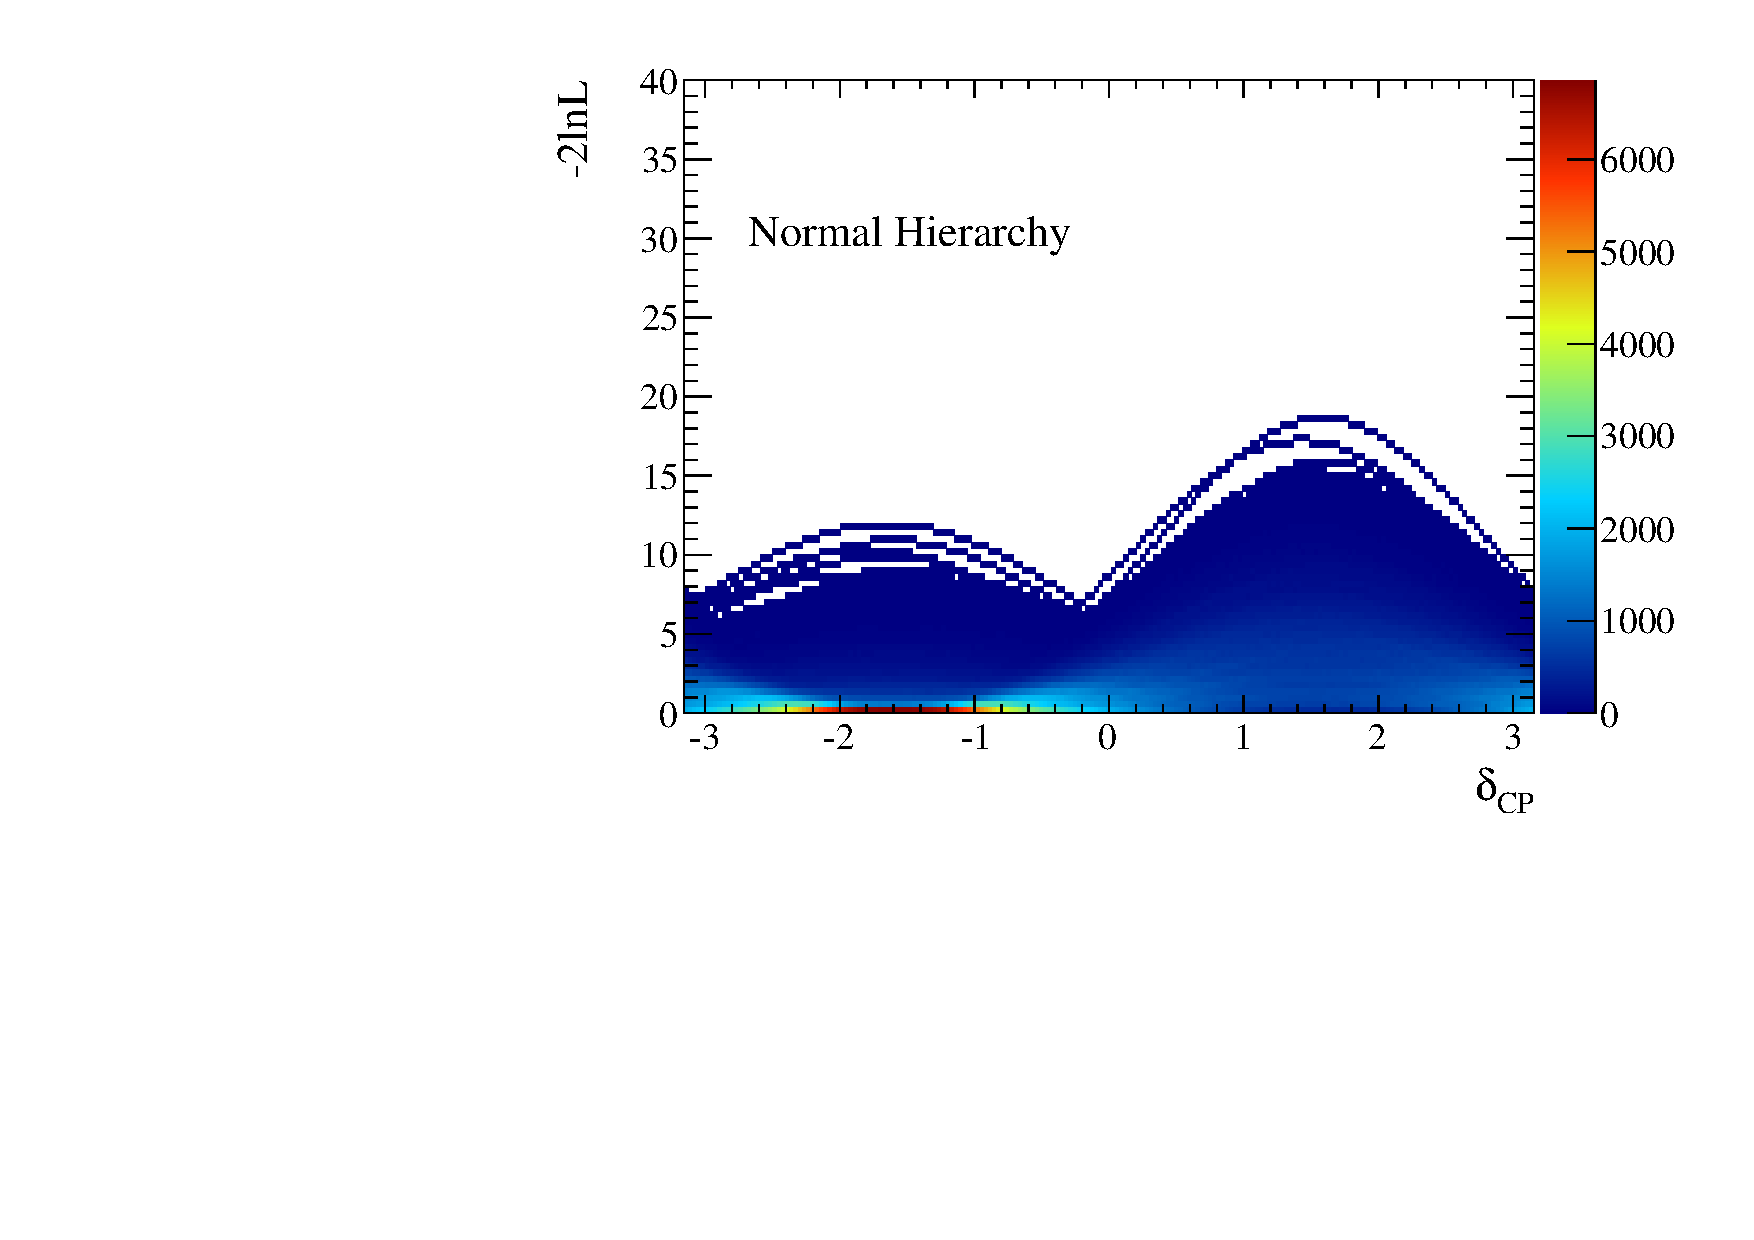
\includegraphics[width=0.9\textwidth]{joint_plots/brazilian_plots/Run17c/dcpVsdchisq_nh_dcp_mpiover2_nh.pdf}
\caption{Normal hierarchy}
\label{fig:deltachisqVsdcp_mpiover2_run17c_nh}
\end{subfigure}
\begin{subfigure}[b]{0.49\textwidth}
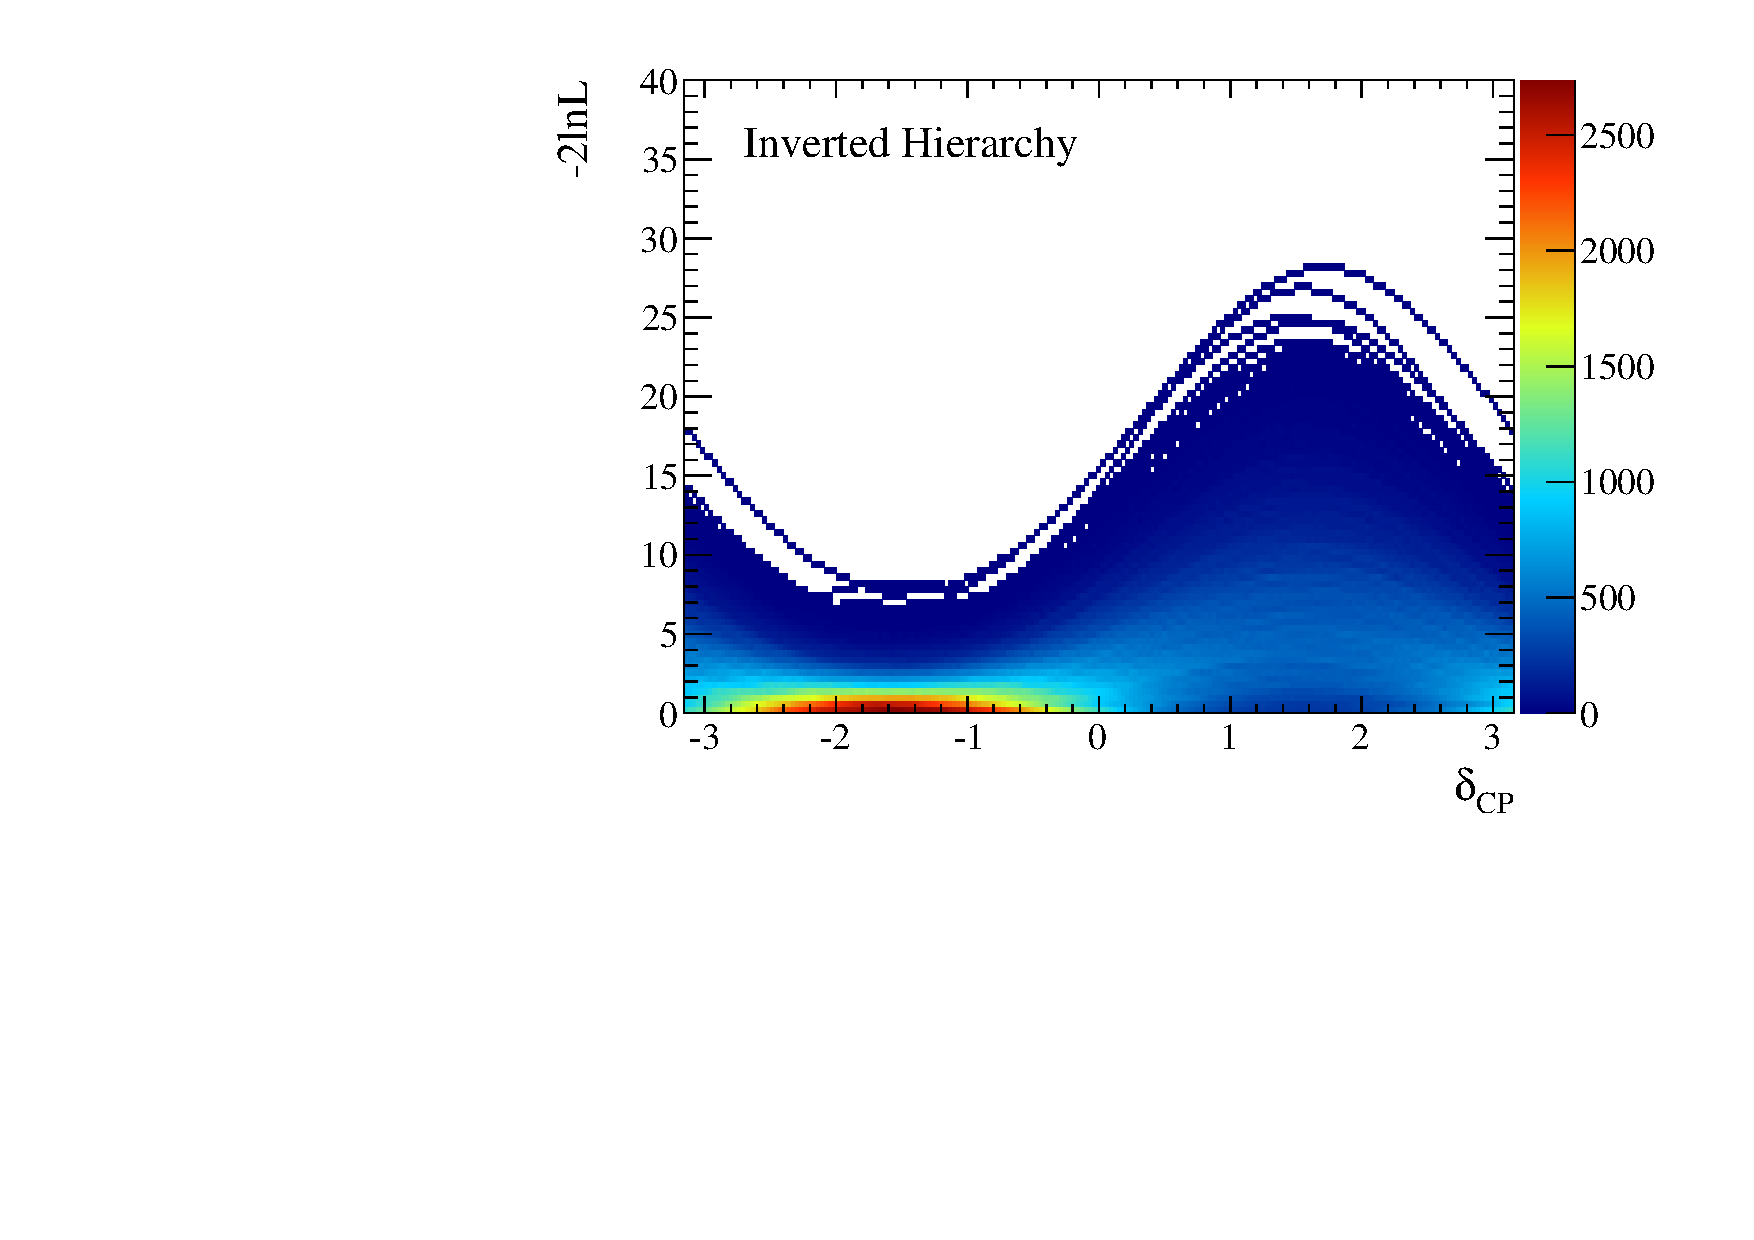
\includegraphics[width=0.9\textwidth]{joint_plots/brazilian_plots/Run17c/dcpVsdchisq_nh_dcp_mpiover2_ih.pdf}
\caption{Inverted hierarchy}
\label{fig:deltachisqVsdcp_mpiover2_run17c_ih}
\end{subfigure}
\caption{
The distribution of $\Delta \chi^2$ vs $\delta_{CP}$ obtained with 10k toy experiments
generated with $\delta_{CP} = -\pi/2$ and normal hierarchy is shown.
The $\Delta \chi^2$ distributions obtained by fixing the mass hierarchy to normal (left)
and inverted (right) are shown.
%The comparison between the expected $<\Delta \chi^2>$ distribution 
%for $\delta_{CP} = -\pi/2$ and normal hierarchy 
%and the Run 1-7c data set $\Delta \chi^2$ distribution is shown.
%10k toy experiments are produced:
%all the oscillation parameters which are not parameters of interest
%are marginalised using the prior distributions shown in \cref{tab:osc_params_joint_priors}
%and applying the reactor constraint.
%The Red solid line is the expected $<\Delta \chi^2>$ distribution.
%The black solid line corresponds to the data $\Delta \chi^2$ distribution.
%The green and yellow bands correspond to the $1\sigma$ and $2\sigma$ 
%uncertainty on the expected $<\Delta \chi^2>$ distribution and
%contain respectively the 68.27c\% and 95.45\% of toy experiments,
%assuming the $\Delta \chi^2$ p.d.f. to be 1-sided.
%The critical values, obtained with the Feldman-Cousins method,
%that define the 90\% (blue) and $2\sigma$ (violet) confidence intervals
%are shown as well.
}
\label{fig:deltachisqVsdcp_mpiover2_run17c}
\end{figure*}


The results are similar to the Run 1-7b one, 
though the Run 1-7c $\Delta \chi^2$ distribution for normal hierarchy is within the $2\sigma$ 
for all the range of $\delta_{CP}$.
Also the Run 1-7c $\Delta \chi^2$ distribution for inverted hierarchy is always within the $2\sigma$ sensitivity region.
The Run 1-7c data set shows a weaker tension with the expectation of the PMNS matrix with $\delta_{CP} = -\pi/2$ and normal hierarchy. 

%It is interesting to note that if the hierarchy is normal there is a non negligible amount
%of toy experiments which best-fit moves far from the true point.
%This becomes clear by looking to the wide peak in the yellow band at $\delta_{CP} = - \pi/2$
%that is due to extreme statistical and/or systematic fluctuations
%the increase the number of events in the antineutrino $e$-like sample
%and decrease the number of events in the neutrino $e$-like sample,
%moving the best-fit to $\delta_{CP} = +\pi/2$ and inverted hierarchy.
%This wide peak is not present in the inverted hierarchy case, because 
%even more extreme fluctuations are needed in order to move the best-fit from 
%$\delta_{CP} = -\pi/2$ to $+\pi/2$. \\

\begin{figure*}[htb]
\center
\begin{subfigure}[b]{0.49\textwidth}
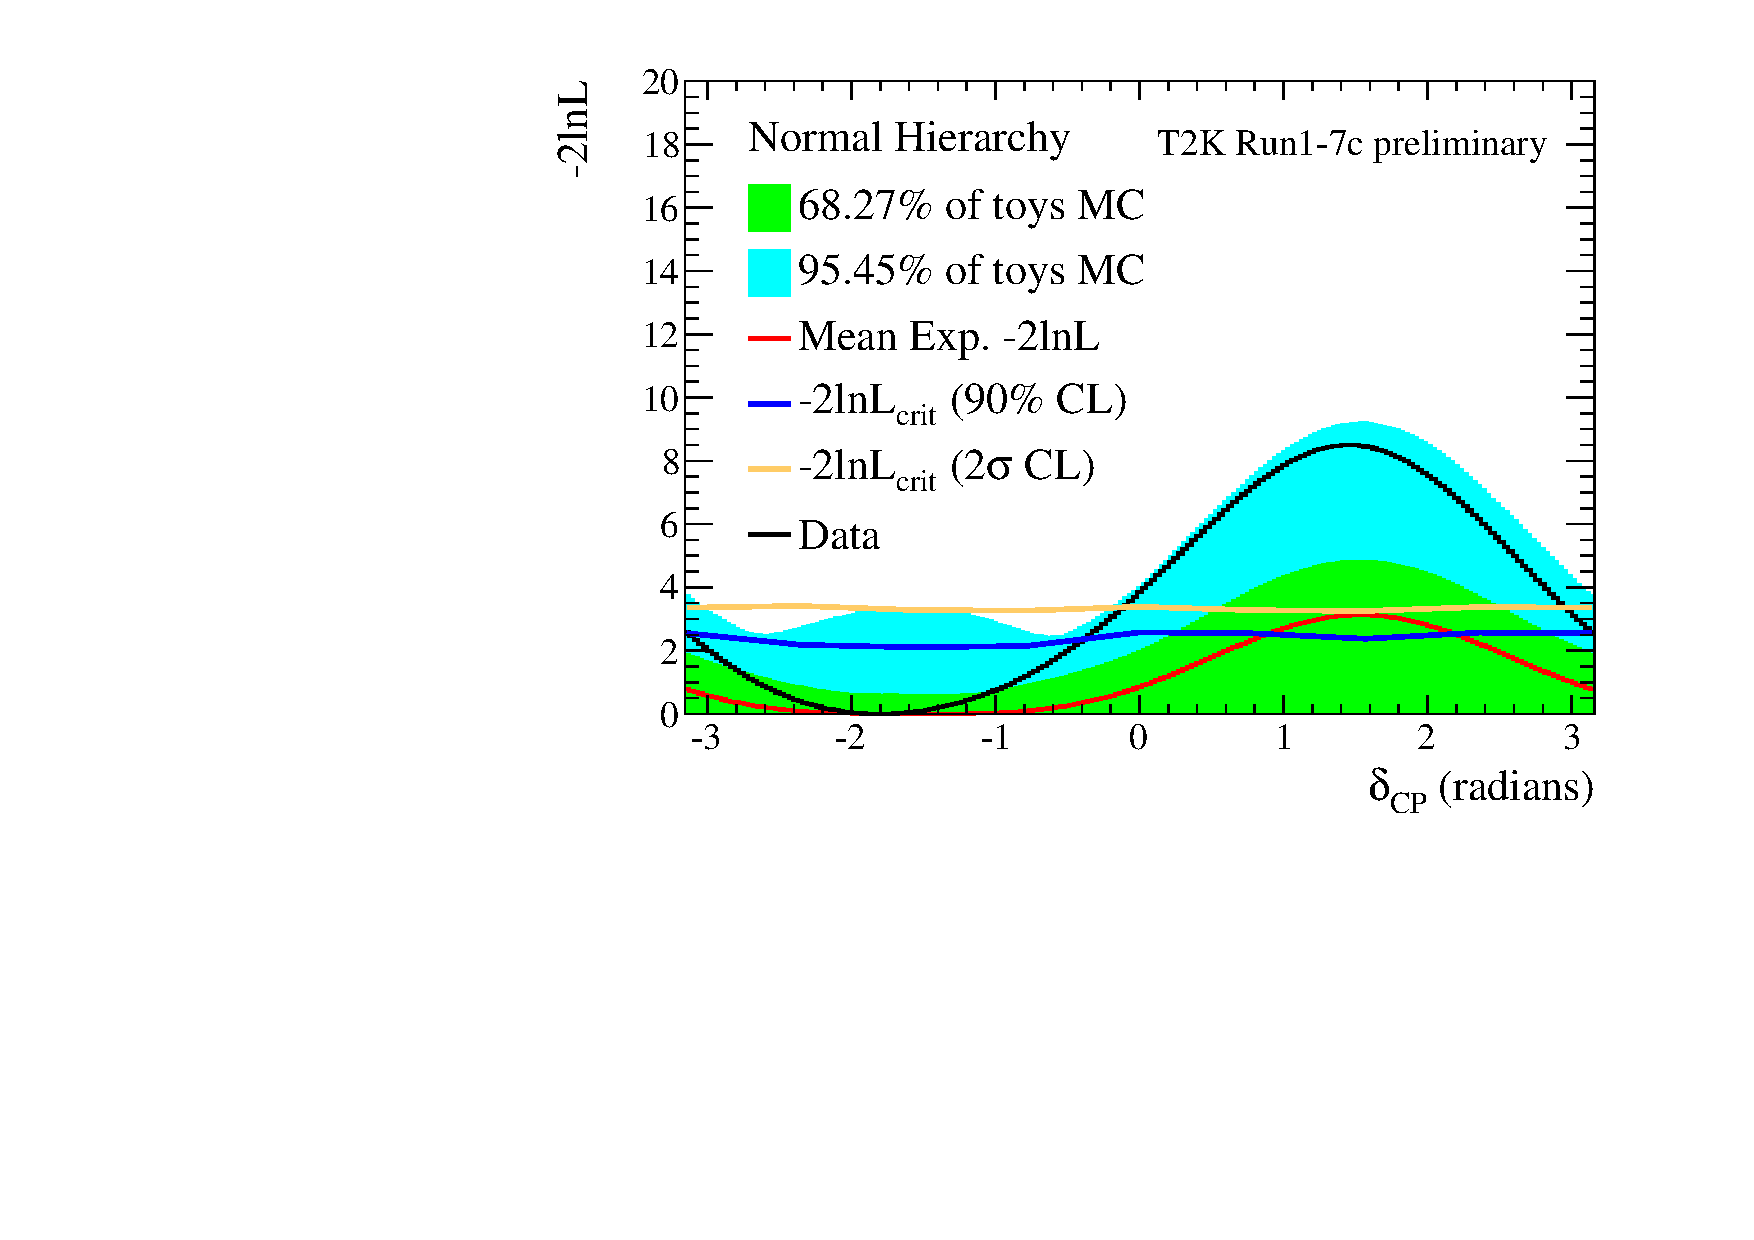
\includegraphics[width=0.9\textwidth]{joint_plots/brazilian_plots/Run17c/brazilian_nh_dcp_mpiover2_run17.pdf}
\caption{Normal hierarchy}
\label{fig:brazilian_mpiover2_run17c_nh}
\end{subfigure}
\begin{subfigure}[b]{0.49\textwidth}
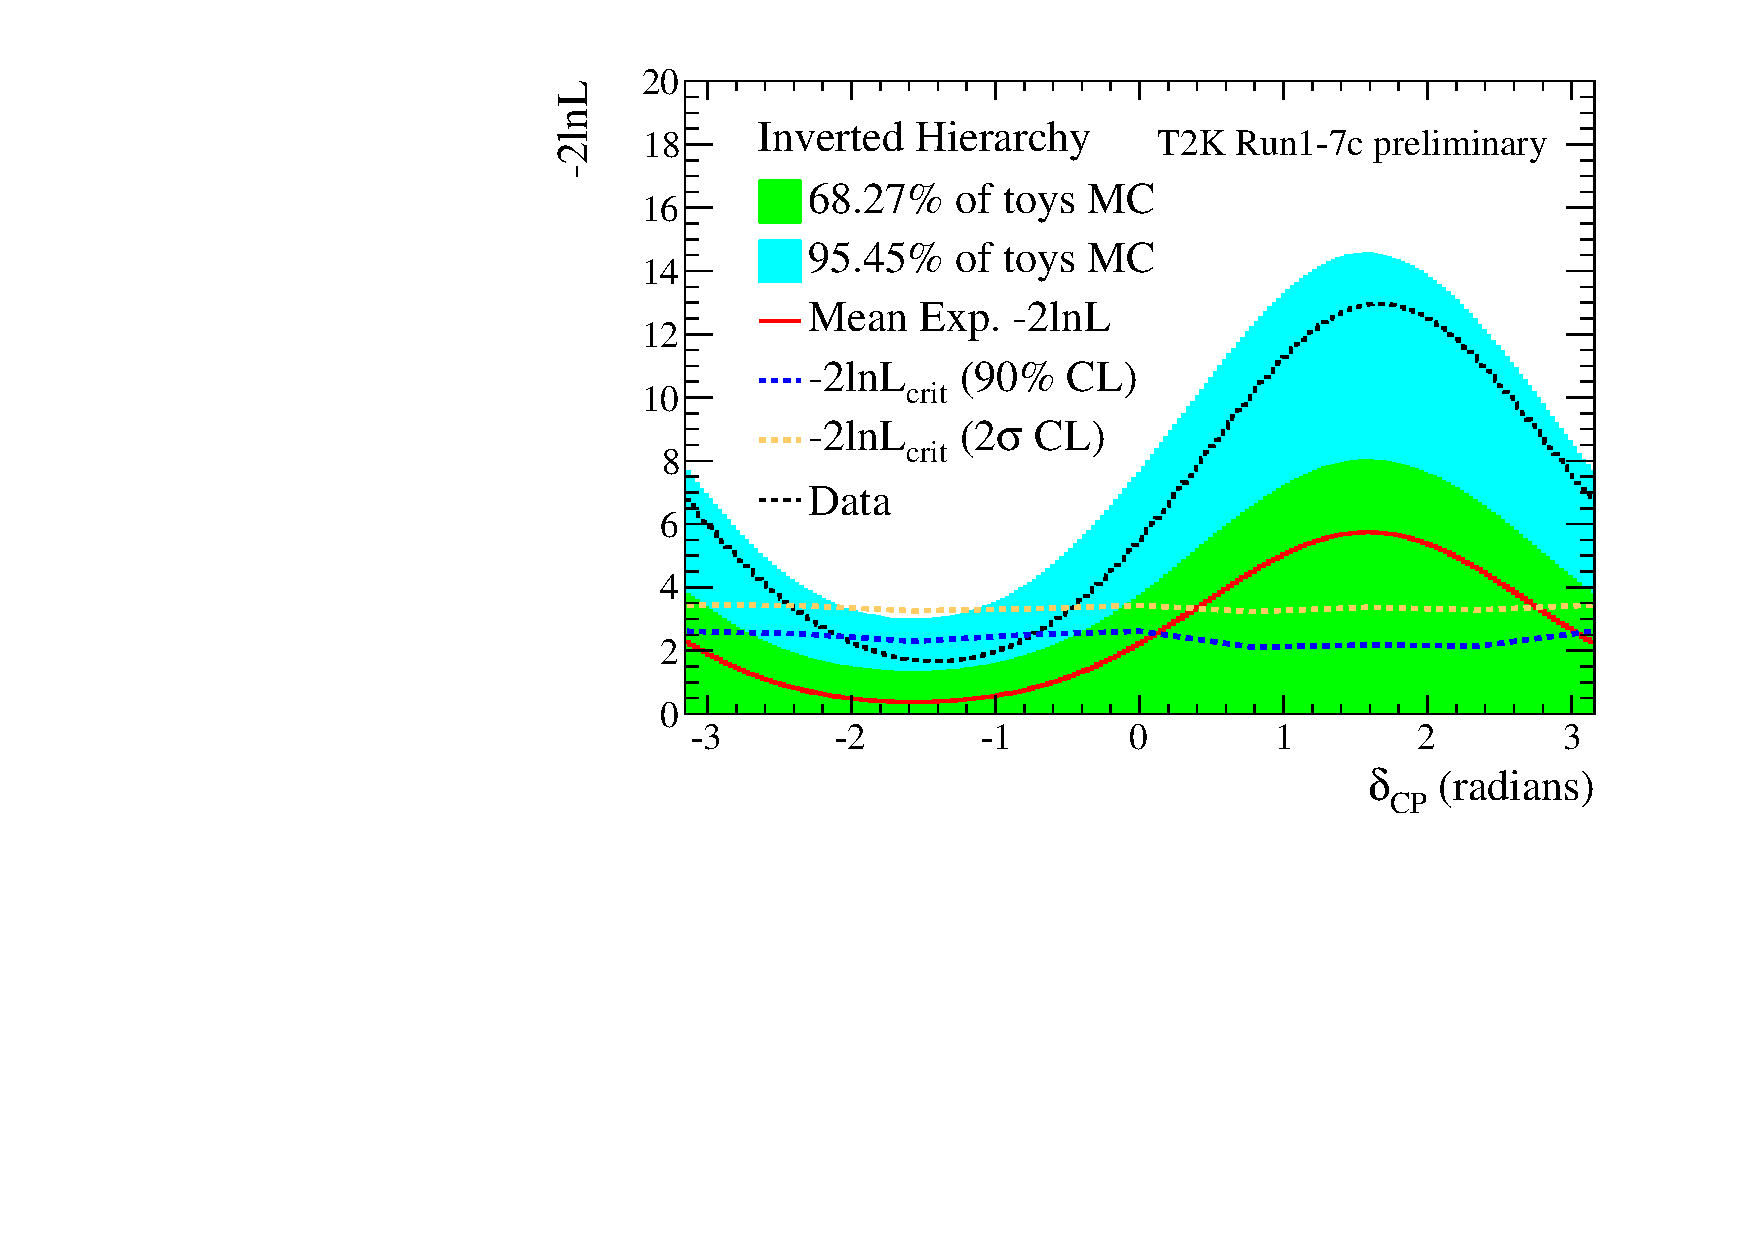
\includegraphics[width=0.9\textwidth]{joint_plots/brazilian_plots/Run17c/brazilian_ih_dcp_mpiover2_run17.pdf}
\caption{Inverted hierarchy}
\label{fig:brazilian_mpiover2_run17c_ih}
\end{subfigure}
\caption{
The comparison between the expected $<\Delta \chi^2>$ distribution 
for $\delta_{CP} = -\pi/2$ and normal hierarchy 
and the Run 1-7c data set $\Delta \chi^2$ distribution is shown.
10k toy experiments are produced:
all the oscillation parameters which are not parameters of interest
are marginalised using the prior distributions shown in \cref{tab:osc_params_joint_priors}
and applying the reactor constraint.
The red solid line is the expected $<\Delta \chi^2>$ distribution.
The black solid line corresponds to the data $\Delta \chi^2$ distribution.
The green and light blue bands correspond to the regions
that contain respectively 68.27\% and 95.45\% of toy experiments
assuming the $\Delta \chi^2$ p.d.f. to be 1-sided.
The critical values, obtained with the Feldman-Cousins method,
that define the 90\% (blue) and $2\sigma$ (orange) confidence intervals
are shown as well.
}
\label{fig:brazilian_mpiover2_run17c}
\end{figure*}


%In \cref{fig:brazilian_pvalue_mpiover2_run17c} the compatibility between data 
%and expected $\Delta \chi^2$ distributions, 
%given $\delta_{CP} = -\pi/2$ and normal hierarchy as true,
%is shown as a p-value and Z-score.
%For each bin of $\delta_{CP}$ and mass hierarchy the $\Delta \chi^2_{bin}$ distribution
%was taken and the p-value was calculated using the $\Delta \chi^2$ value in that 
%bin of $\delta_{CP}$ and mass hierarchy obtained from the Run 1-7c data set fit.
%Consequently the Z-score was computed as described in 
%appendix~\ref{app:method_significance}.
%This p-value shows how much the Run 1-7c data set 
%is consistent with the expected $\Delta \chi^2$ distribution
%as a function of $\delta_{CP}$ and mass hierarchy,
%if Nature is $\delta_{CP} = -\pi/2$ and normal hierarchy.
%We can see that for most of the range of $\delta_{CP}$ and mass hierarchy
%the Run 1-7c data set is consistent with $\delta_{CP} = -\pi/2$ and normal hierarchy
%within $2\sigma$, except the regions $\{0,2\}$ for normal hierarchy 
%and $\{2,3\}$ for inverted hierarchy, which are not consistent at about $2-2.2 \sigma$ level.
%This plot is another way, quantitative, to compare data and expected
%$\Delta \chi^2$ distributions of \cref{fig:brazilian_mpiover2_run17c}.
%
%\begin{figure*}[htb]
%\center
%\begin{subfigure}[b]{0.49\textwidth}
%\includegraphics[width=0.9\textwidth]{joint_plots/brazilian_plots/Run17c/pvalue_data_sensi_mpiover2_run17.pdf}
%\caption{P-value}
%\label{fig:brazilian_mpiover2_run17c_nh}
%\end{subfigure}
%\begin{subfigure}[b]{0.49\textwidth}
%\includegraphics[width=0.9\textwidth]{joint_plots/brazilian_plots/Run17/zscore_data_sensi_mpiover2_run17.pdf}
%\caption{Z-score}
%\label{fig:brazilian_mpiover2_run17_ih}
%\end{subfigure}
%\caption{
%P-value (left) and Z-score for consistency of the Run 1-7 data set
%with the expected $<\Delta \chi^2>$ distribution given the true values
%$\delta_{CP} = -\pi/2$ and normal hierarchy.
%}
%\label{fig:brazilian_pvalue_mpiover2_run17}
%\end{figure*}


In \cref{fig:prob_exclusion_mpiover2_run17c} 
the probability to exclude $\delta_{CP}$ at 90\% (black) and $2\sigma$ (red) CL, 
if nature is $\delta_{CP}=-\pi/2$ and normal hierarchy, is shown
for both normal (solid line) and inverted (dashed line) hierarchy.
%This is a MC only study obtained with 10k toy experiments using
%the same procedure as described above.
%In this case the probability is defined as the number of toy experiments
%that satisfies the condition $\Delta \chi^2_{bin} > \Delta \chi^2_{crit}$
%divided by the total number of toy experiments,
%where the critical values were computed using the Feldman-Cousins method
%(see \cref{fig:joint_dcp_fc_run17c}).
It is shown that the fraction of toy experiments that exclude $\delta_{CP}=0$
with a significance of $2\sigma$,
which is the case of the Run 1-7c data set,  
is about 9.2\%
for normal hierarchy and about 35.5\% for inverted hierarchy.
It is also interesting to see that the 
number of toy experiments that exclude $\delta_{CP} = \pi$
at 90\% CL is about 17.3\% for normal hierarchy.

\begin{figure*}[htb]
\center
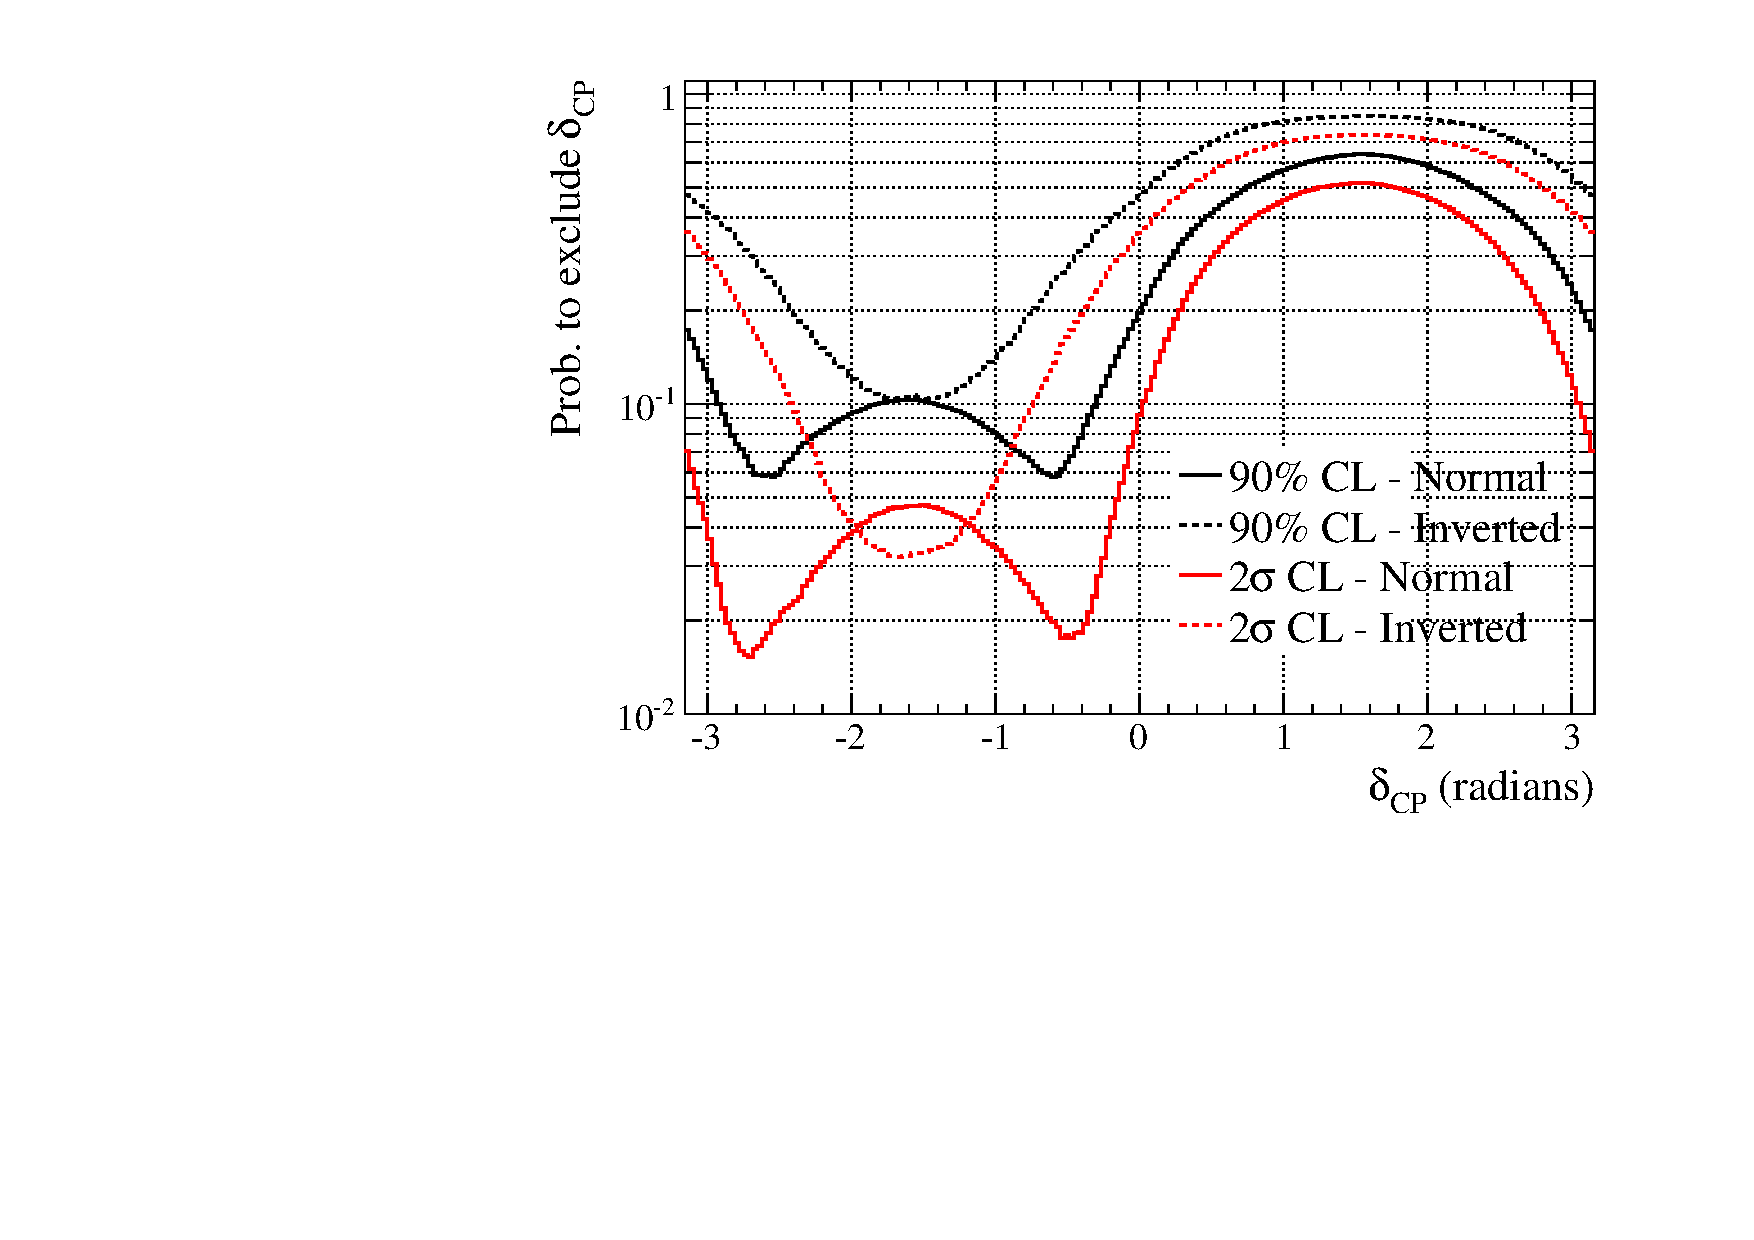
\includegraphics[width=0.49\textwidth]{joint_plots/brazilian_plots/Run17c/prob_excl_dcp_mpiover2_run17.pdf}
\caption{
The number of toy experiments that exclude $\delta_{CP}$ at 90\% (black) and $2\sigma$ (red) CL, 
if nature is $\delta_{CP}=-\pi/2$ and normal hierarchy, is shown
for both normal (solid line) and inverted (dashed line) hierarchy.
}
\label{fig:prob_exclusion_mpiover2_run17c}
\end{figure*}

%In appendix~\ref{app:brazilian_asimov_mean_dcp_run17c} the comparison between 
%mean and Asimov data set A sensitivity for Run 1-7c is shown.
%The same procedure as described above is used, 
%by replacing the Run 1-7c data set $\Delta \chi^2$ distribution with the Asimov data set A one.

\clearpage





\subsubsection {Run 1-7c best-fit: $\delta_{CP} = -1.791$ - normal hierarchy}
\label{sec:dcp_m1p791_nh_run17c}

The same study as in \cref{sec:dcp_mpiover2_nh_run17c} is
done for 
the Run 1-7c best-fit point:
$\delta_{CP} = -1.791$ and normal hierarchy.
The result is very similar to the one
for 
$\delta_{CP} = -\pi/2$ and normal hierarchy.

\begin{figure*}[htb]
\center
\begin{subfigure}[b]{0.49\textwidth}
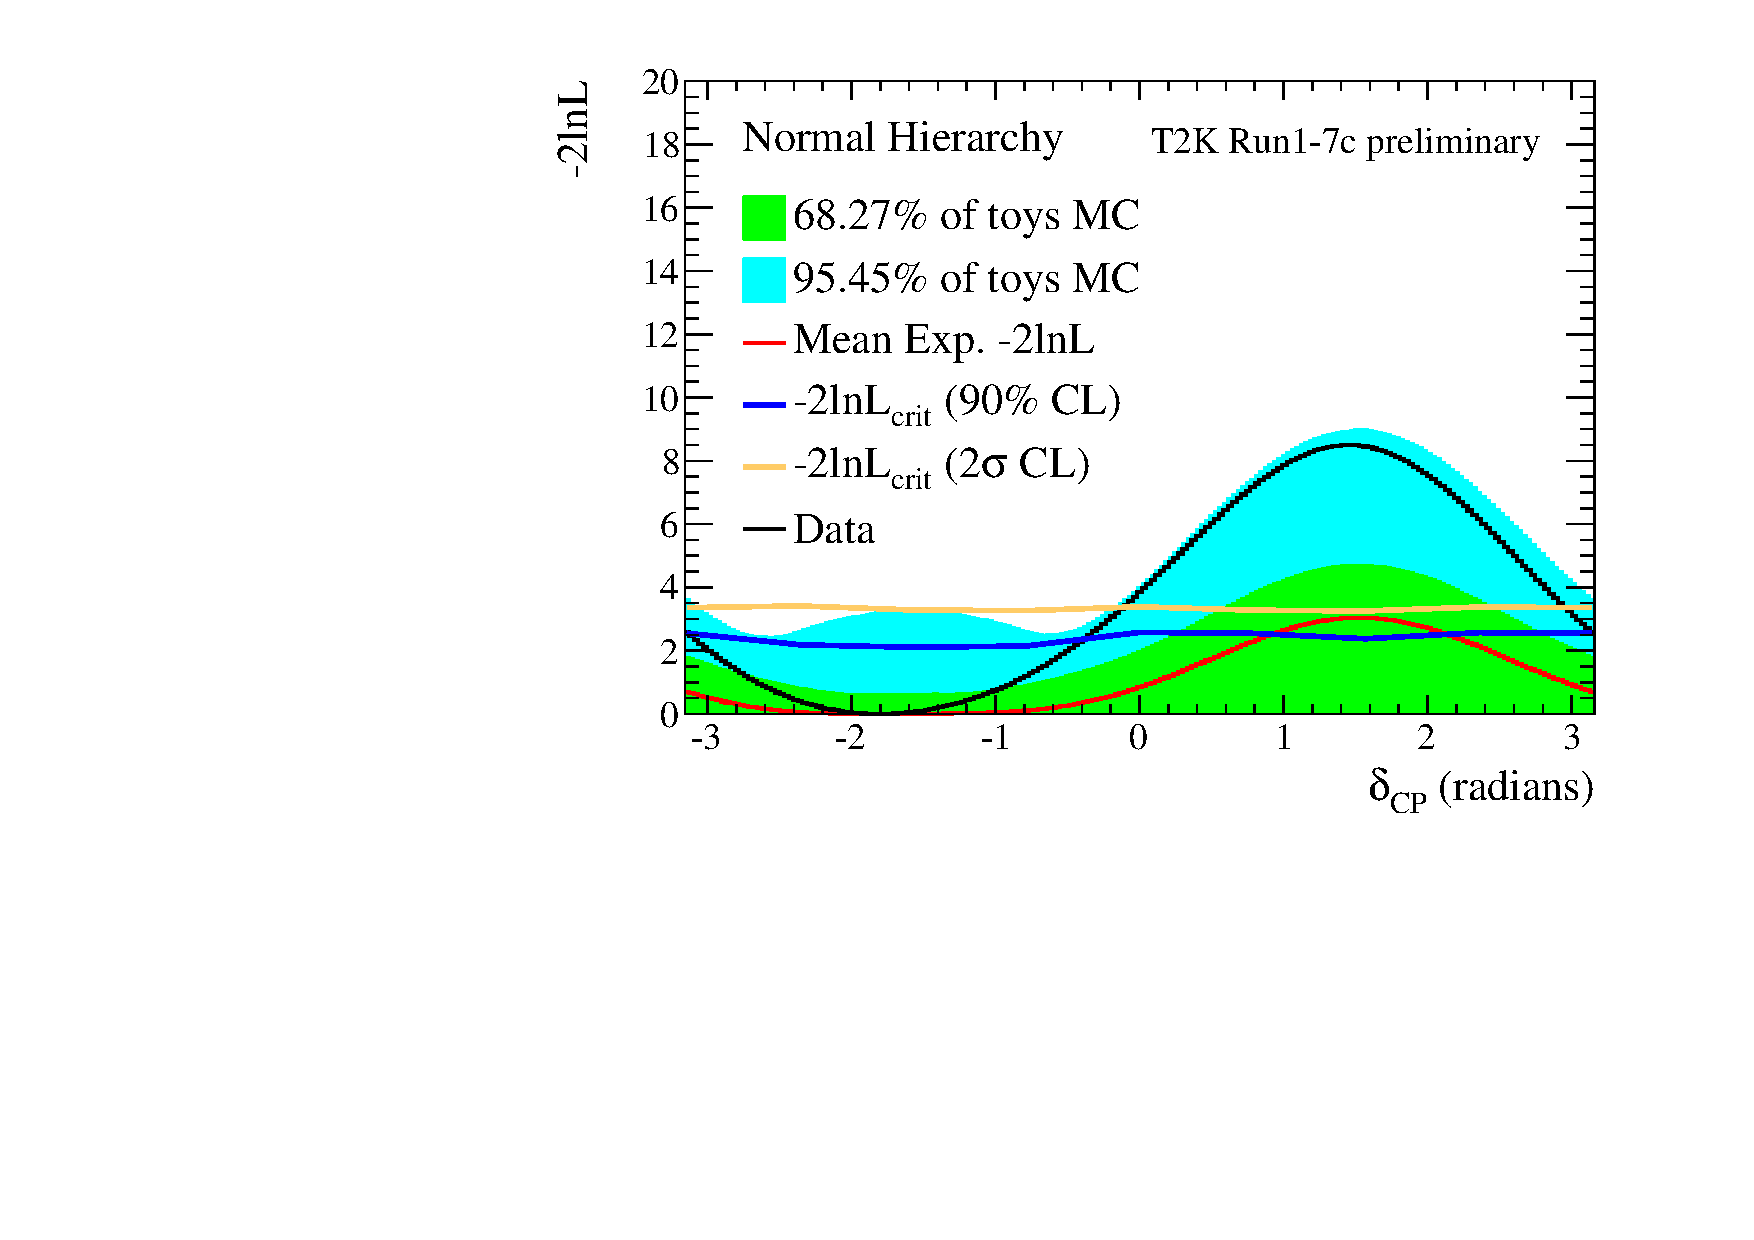
\includegraphics[width=0.9\textwidth]{joint_plots/brazilian_plots/Run17c/brazilian_nh_dcp_m1p791_run17.pdf}
\caption{Normal hierarchy}
\label{fig:brazilian_m1p791_run17c_nh}
\end{subfigure}
\begin{subfigure}[b]{0.49\textwidth}
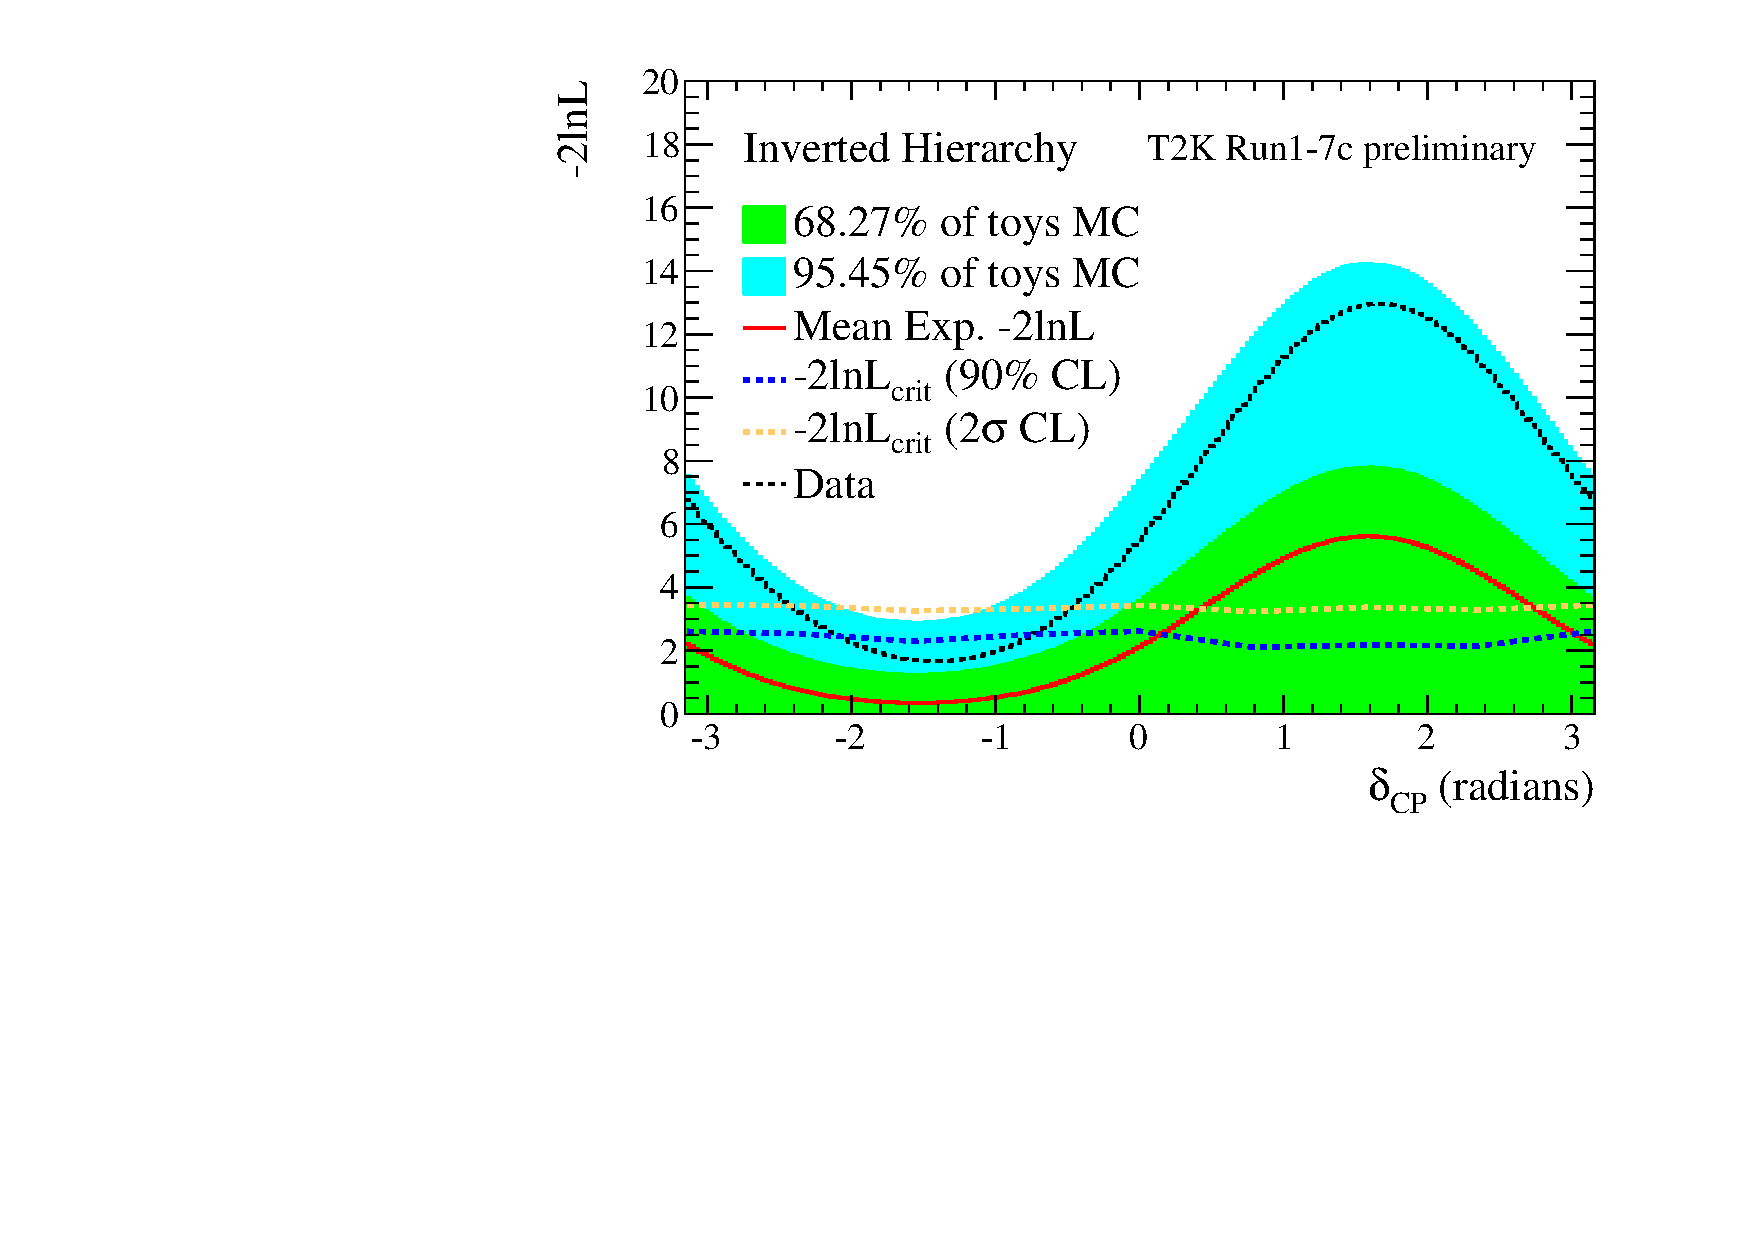
\includegraphics[width=0.9\textwidth]{joint_plots/brazilian_plots/Run17c/brazilian_ih_dcp_m1p791_run17.pdf}
\caption{Inverted hierarchy}
\label{fig:brazilian_m1p791_run17c_ih}
\end{subfigure}
\caption{
The comparison between the expected $<\Delta \chi^2>$ distribution 
for $\delta_{CP} = -1.791$ and normal hierarchy (Run 1-7c best-fit)
and the Run 1-7c data set $\Delta \chi^2$ distribution is shown.
10k toy experiments are produced:
all the oscillation parameters which are not parameters of interest
are marginalised using the prior distributions shown in \cref{tab:osc_params_joint_priors}
and applying the reactor constraint.
The red solid line is the expected $<\Delta \chi^2>$ distribution.
The black solid line corresponds to the data $\Delta \chi^2$ distribution.
The green and light blue bands correspond to the regions
that contain respectively 68.27\% and 95.45\% of toy experiments
assuming the $\Delta \chi^2$ p.d.f. to be 1-sided.
The critical values, obtained with the Feldman-Cousins method,
that define the 90\% (blue) and $2\sigma$ (orange) confidence intervals
are shown as well.}
\label{fig:brazilian_m1p791_run17c}
\end{figure*}


\begin{figure*}[htb]
\center
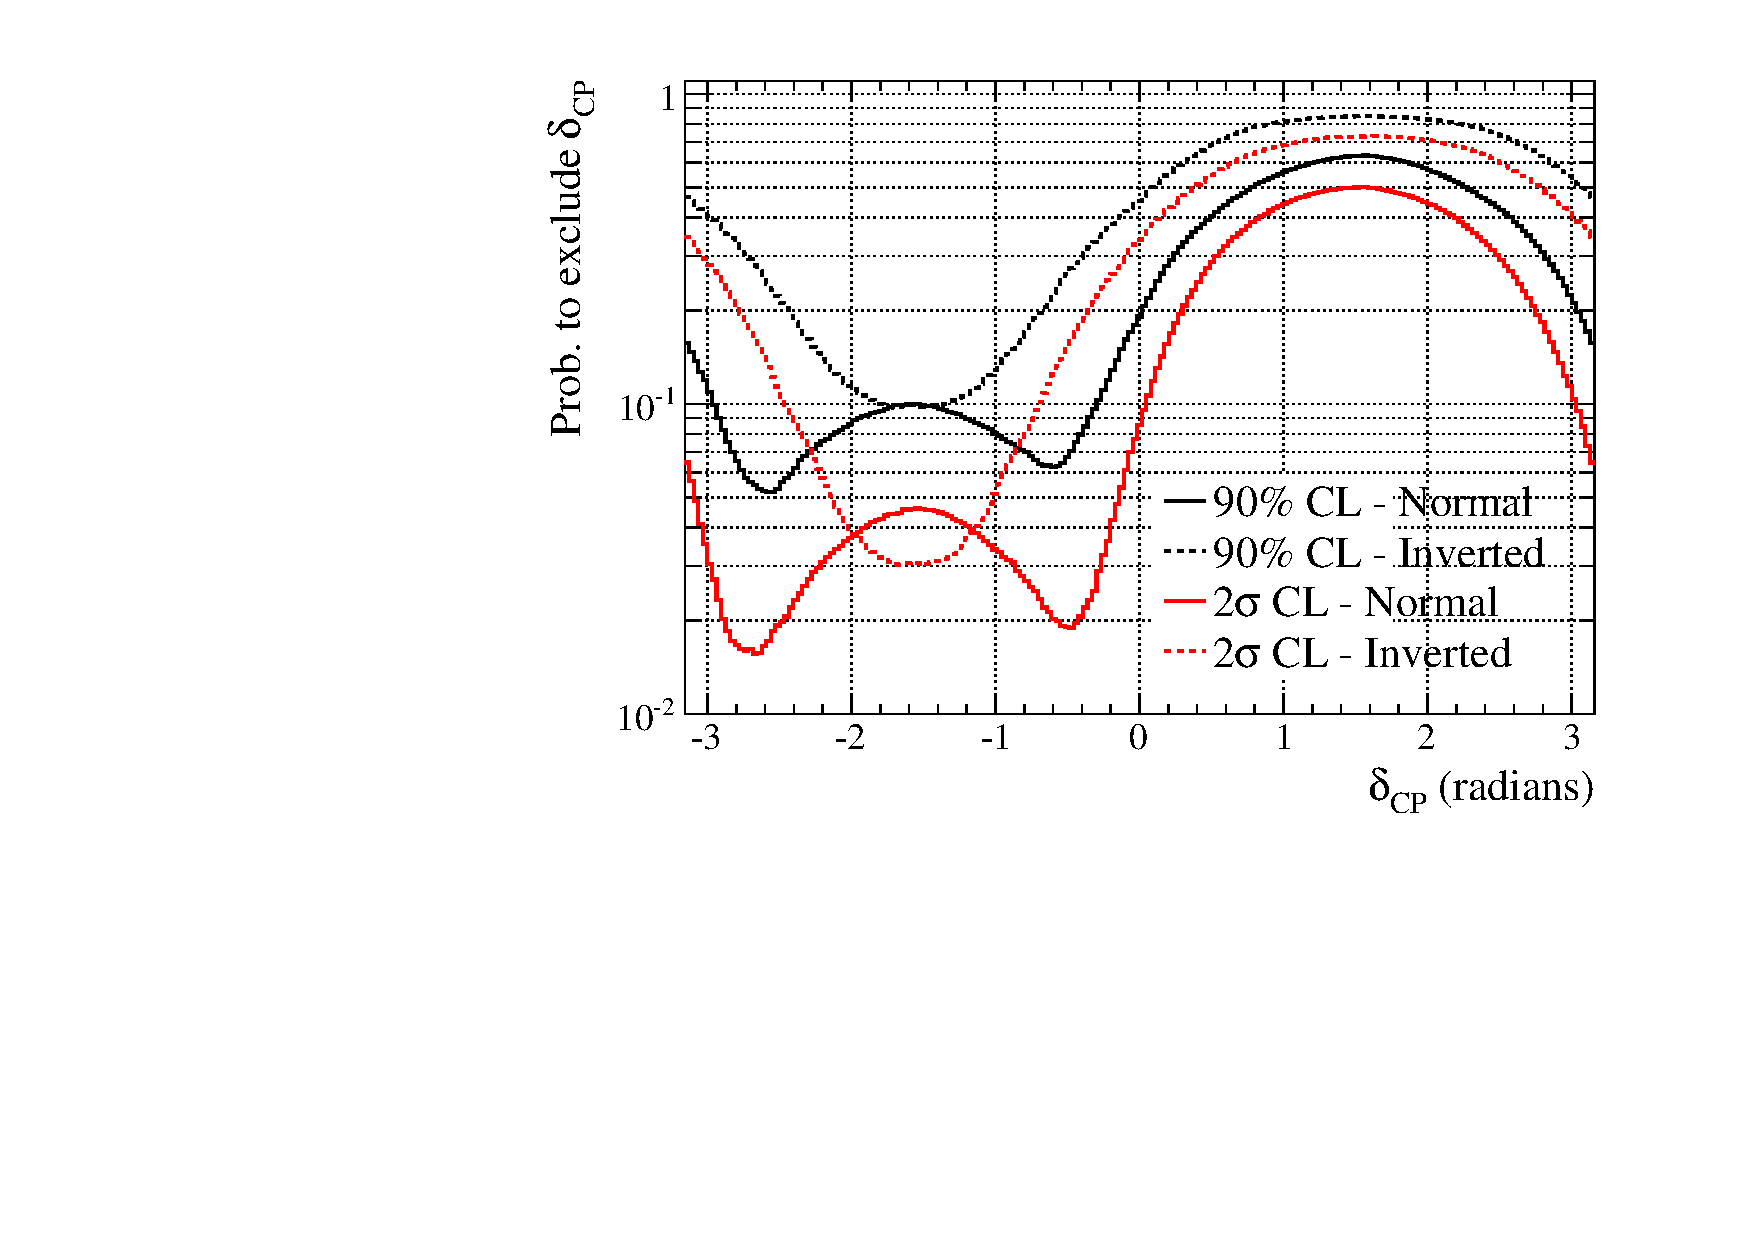
\includegraphics[width=0.49\textwidth]{joint_plots/brazilian_plots/Run17c/prob_excl_dcp_m1p791_run17.pdf}
\caption{
The number of toy experiments that exclude $\delta_{CP}$ at 90\% (black) and $2\sigma$ (red) CL, 
if nature is $\delta_{CP}=-1.791$ and normal hierarchy, is shown
for both normal (solid line) and inverted (dashed line) hierarchy.
}
\label{fig:prob_exclusion_m1p791_run17c}
\end{figure*}


\clearpage










\subsubsection {$\delta_{CP} = 0$ - normal hierarchy}
\label{sec:dcp_0_nh_run17c}

The same study as in \cref{sec:dcp_mpiover2_nh_run17c} is
done for 
$\delta_{CP} = 0$ and normal hierarchy,
i.e. CP is conserved.

From \cref{fig:brazilian_0_run17c} it is clear that the Run 1-7c data set 
is not consistent with the hypothesis of $\delta_{CP} = 0$ and normal hierarchy
for both hierarchy cases.
 
\begin{figure*}[htb]
\center
\begin{subfigure}[b]{0.49\textwidth}
%
\includegraphics[width=0.9\textwidth]{./images/missing_plot-eps-converted-to.pdf}
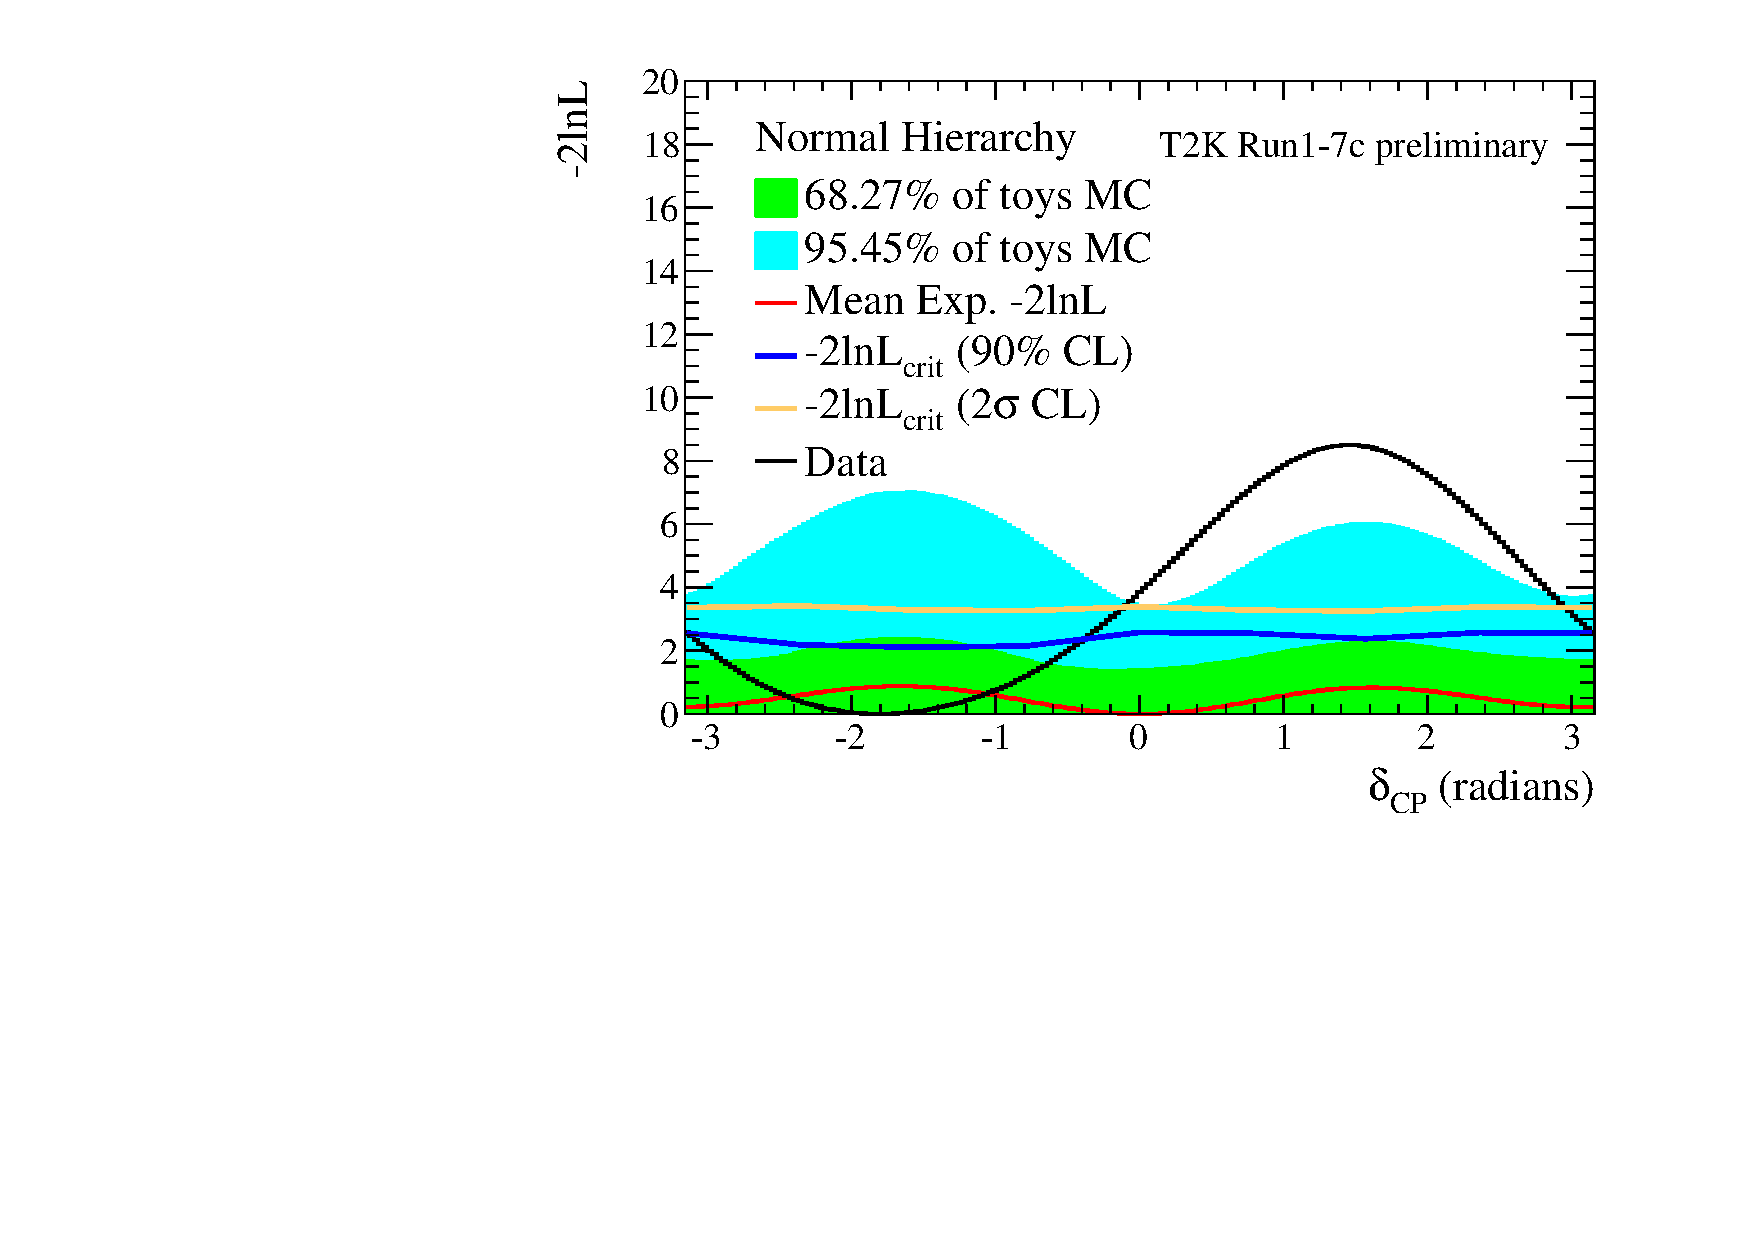
\includegraphics[width=0.9\textwidth]{joint_plots/brazilian_plots/Run17c/brazilian_nh_dcp_0_run17.pdf}
\caption{Normal hierarchy}
\label{fig:brazilian_0_run17c_nh}
\end{subfigure}
\begin{subfigure}[b]{0.49\textwidth}
%
\includegraphics[width=0.9\textwidth]{./images/missing_plot-eps-converted-to.pdf}
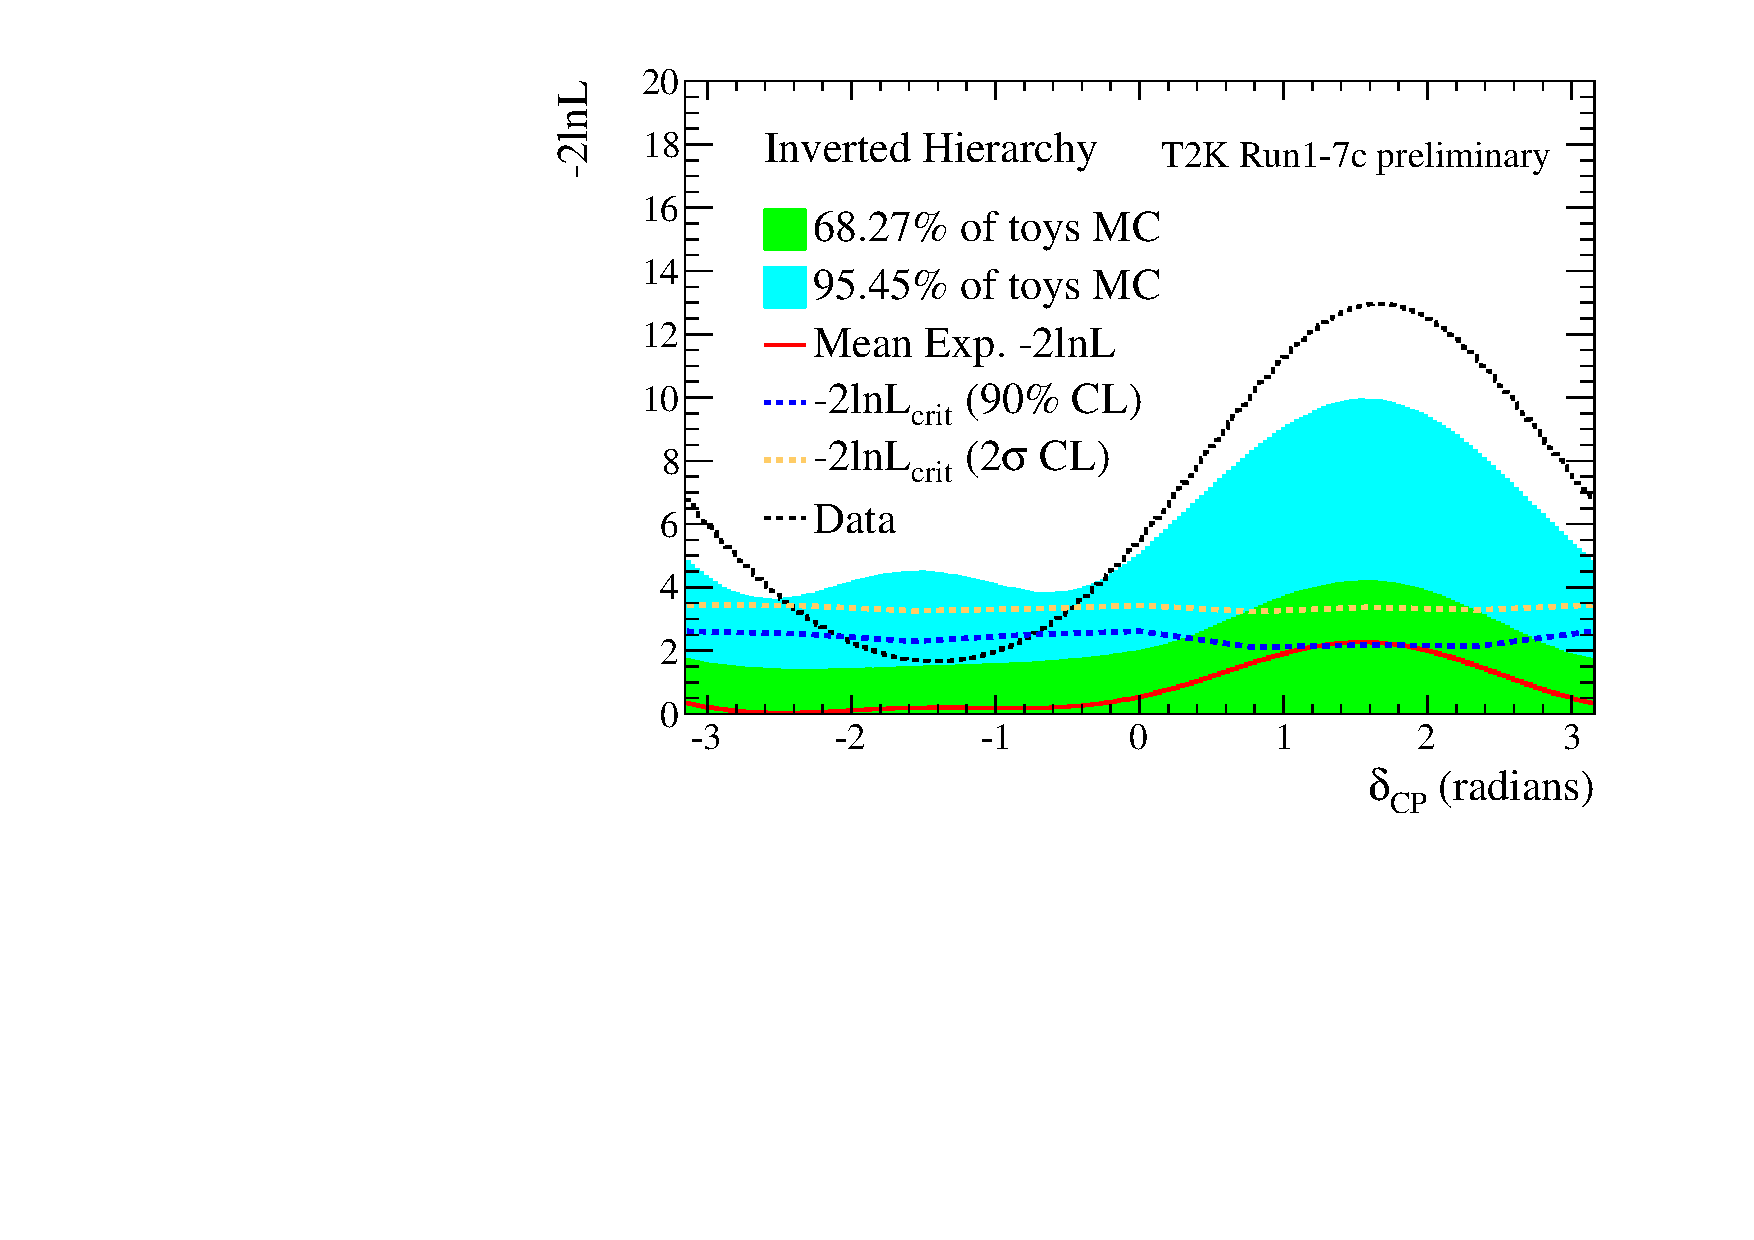
\includegraphics[width=0.9\textwidth]{joint_plots/brazilian_plots/Run17c/brazilian_ih_dcp_0_run17.pdf}
\caption{Inverted hierarchy}
\label{fig:brazilian_0_run17c_ih}
\end{subfigure}
\caption{
The comparison between the expected $<\Delta \chi^2>$ distribution 
for $\delta_{CP} = 0$ and normal hierarchy
and the Run 1-7c data set $\Delta \chi^2$ distribution is shown.
10k toy experiments are produced:
all the oscillation parameters which are not parameters of interest
are marginalised using the prior distributions shown in \cref{tab:osc_params_joint_priors}
and applying the reactor constraint.
The red solid line is the expected $<\Delta \chi^2>$ distribution.
The black solid line corresponds to the data $\Delta \chi^2$ distribution.
The green and light blue bands correspond to the regions
that contain respectively 68.27\% and 95.45\% of toy experiments
assuming the $\Delta \chi^2$ p.d.f. to be 1-sided.
The critical values, obtained with the Feldman-Cousins method,
that define the 90\% (blue) and $2\sigma$ (orange) confidence intervals
are shown as well.
}
\label{fig:brazilian_0_run17c}
\end{figure*}

%Since the p-value that shows the consistency of the Run 1-7c $\Delta \chi^2$ 
%with the hypothesis of $\delta_{CP} = 0$ and normal hierarchy is 
%low (close to $3 \sigma$) and 10k toy experiments are not enough
%to reach a good precision 
%and more CPU time is needed.
%So the p-value and Z-score as in the previous sections are not shown.
%However \cref{fig:brazilian_0_run17c} is enough to understand the
%consistency of the Run 1-7c data set $\Delta \chi^2$ distribution
%with the expected one.

In \cref{fig:prob_exclusion_0_run17c} it shown that the 
fraction of toy experiments for which $\delta_{CP} = 0$ and normal hierarchy is excluded at $2\sigma$ is
$4.8\%$ 
%(consistent with 4.5\%, i.e. with Feldman-Cousins method,
%within statistical error on the number of toy experiments
%by construction of $\Delta \chi^2_{bin}$ 
%where $bin$ coincides with the $true$ point)
and about 12\% for inverted hierarchy.
The fraction of toy experiments where $\delta_{CP} = \pi$ 
is excluded at 90\% CL is about 14.9\% for normal hierarchy and
about 17.7\% for inverted hierarchy.

\begin{figure*}[htb]
\center
%
\includegraphics[width=0.9\textwidth]{./images/missing_plot-eps-converted-to.pdf}
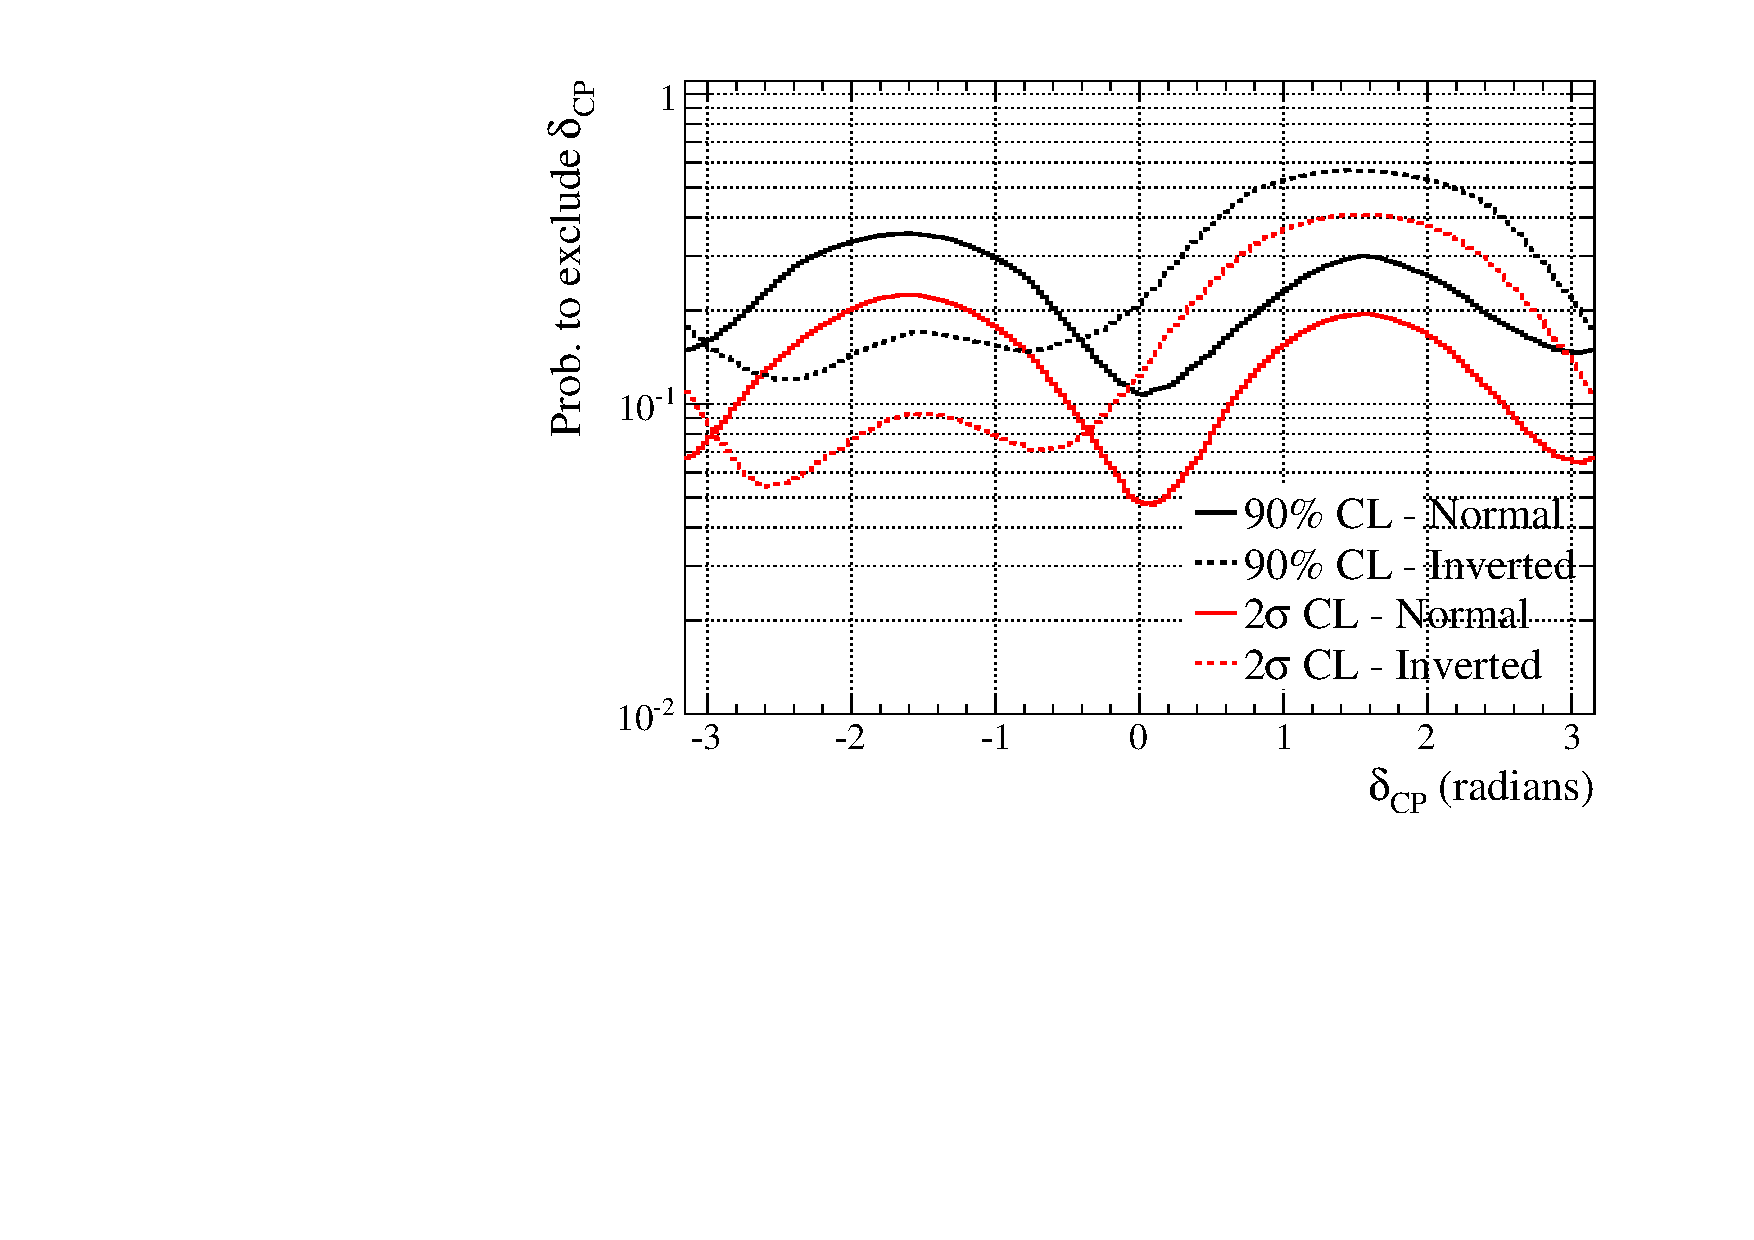
\includegraphics[width=0.49\textwidth]{joint_plots/brazilian_plots/Run17c/prob_excl_dcp_0_run17.pdf}
\caption{
The number of toy experiments that exclude $\delta_{CP}$ at 90\% (black) and $2\sigma$ (red) CL, 
if nature is $\delta_{CP}=0$ and normal hierarchy, is shown
for both normal (solid line) and inverted (dashed line) hierarchy.
}
\label{fig:prob_exclusion_0_run17c}
\end{figure*}


\clearpage







\subsubsection {$\delta_{CP} = -\pi/2$ - inverted hierarchy}
\label{sec:dcp_mpiover_ih_run17c}

The same study as in \cref{sec:dcp_mpiover2_nh_run17c} is
done for 
$\delta_{CP} = -\pi/2$ and inverted hierarchy.

From \cref{fig:brazilian_mpiover2_trueIH_run17c} 
it is clear that $\delta_{CP}$ and mass hierarchy are degenerate and so highly correlated
as shown for the Run 1-7b data set in \cref{sec:dcp_mpiover_ih_run17c}.
%Indeed the expected $\Delta \chi^2$ spread is similar to the one shown in \cref{sec:dcp_0_nh_run17c}
%for $\delta_{CP} = 0$ and normal hierarchy.
%Actually these two points have similar effects in the reconstructed neutrino energy spectra,
%as shown in \cref{fig:mass_hierarchy_MC_shift}:
%inverted hierarchy increases the number of events in antineutrino mode $e$-like sample
%and decreases it in the neutrino mode $e$-like sample, compared to normal hierarchy,
%which is similar to what happens if $\delta_{CP} = 0$ instead of $-\pi/2$.
%For this reason we see see the best-fit value of $\delta_{CP}$ at 0 for normal hierarchy.
%For inverted hierarchy the best-fit value of $\delta_{CP}$ is $-\pi/2$ as the true one.
%Furthermore the inverted hierarchy mean expected $\Delta \chi^2$ distribution is slightly favored
%with respect to the inverted hierarchy one.
 
\begin{figure*}[htb]
\center
\begin{subfigure}[b]{0.49\textwidth}
%
\includegraphics[width=0.9\textwidth]{./images/missing_plot-eps-converted-to.pdf}
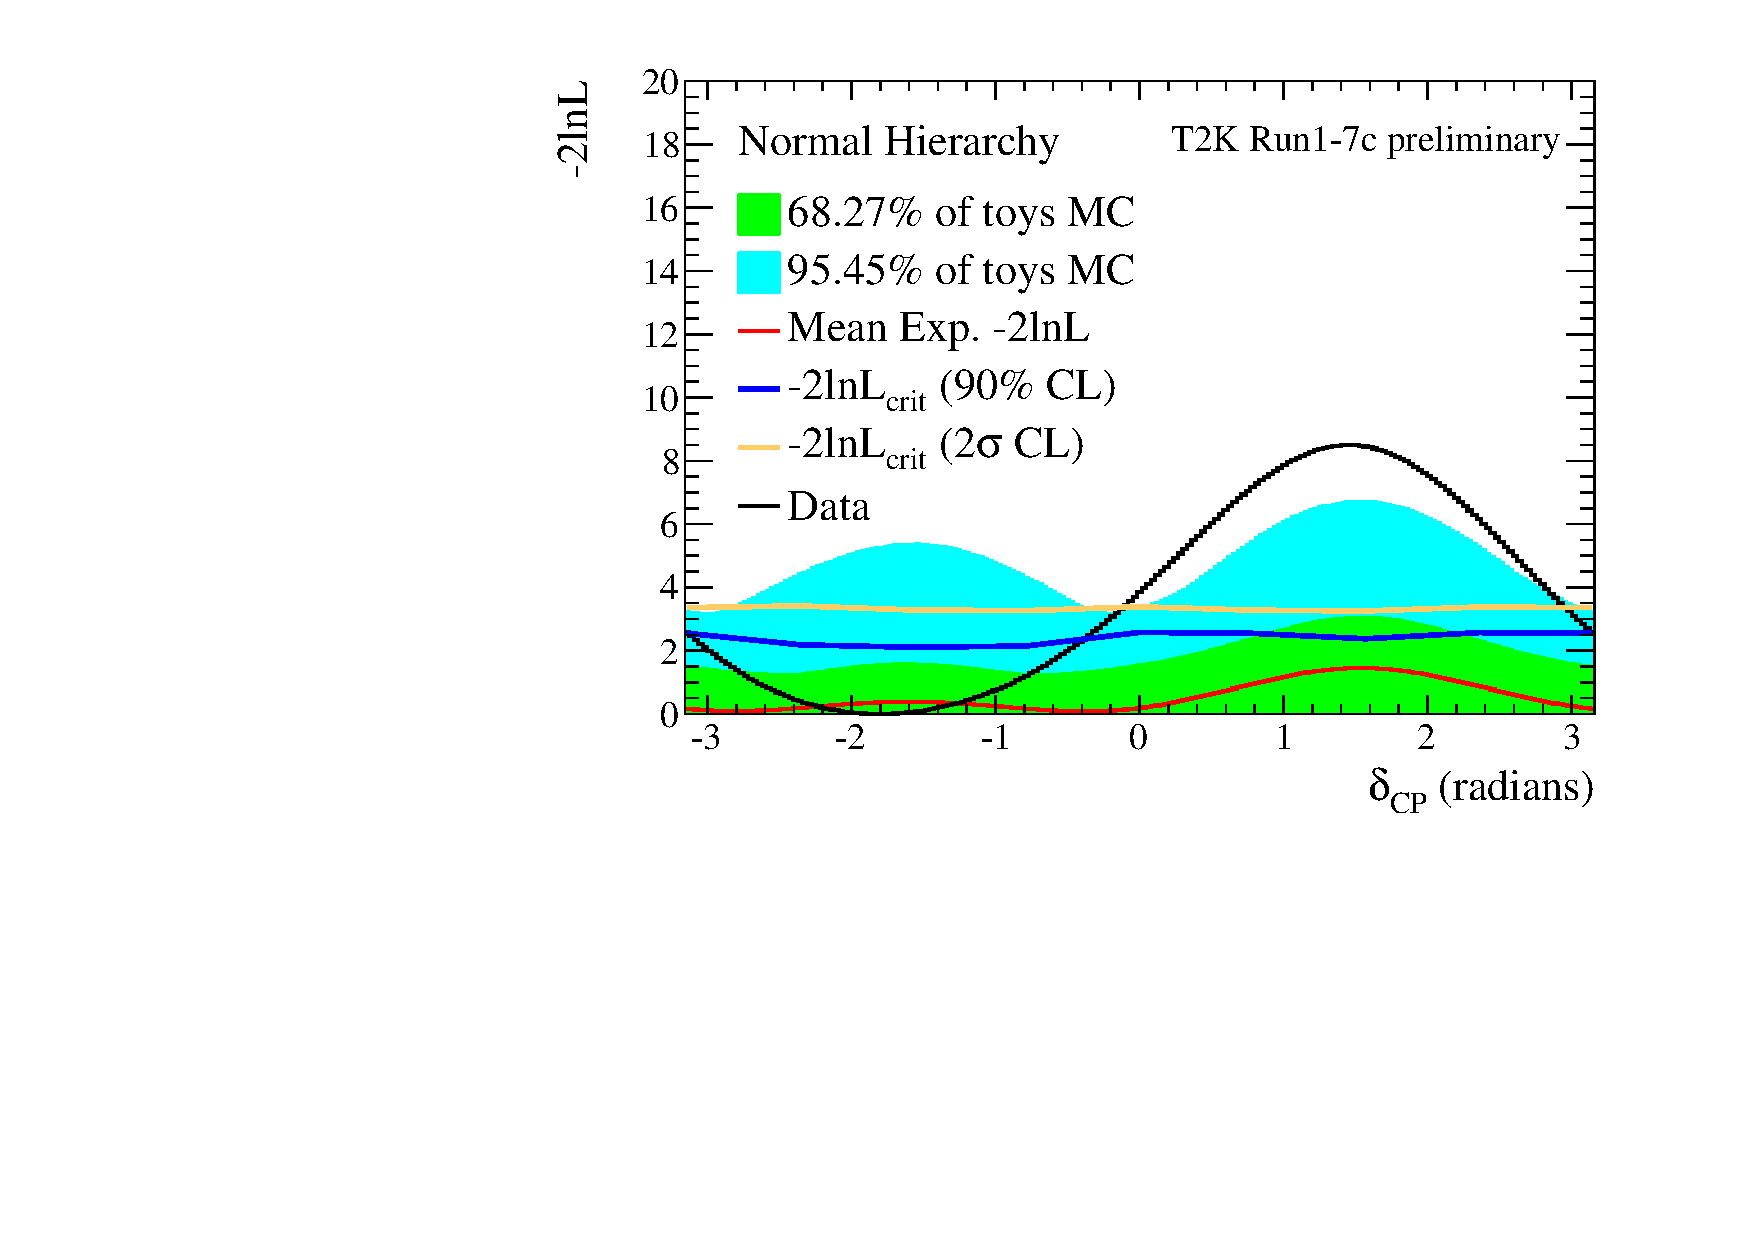
\includegraphics[width=0.9\textwidth]{joint_plots/brazilian_plots/Run17c/brazilian_nh_dcp_mpiover2_trueIH_run17.pdf}
\caption{Normal hierarchy}
\label{fig:brazilian_mpiover2_trueIH_run17c_nh}
\end{subfigure}
\begin{subfigure}[b]{0.49\textwidth}
%
\includegraphics[width=0.9\textwidth]{./images/missing_plot-eps-converted-to.pdf}
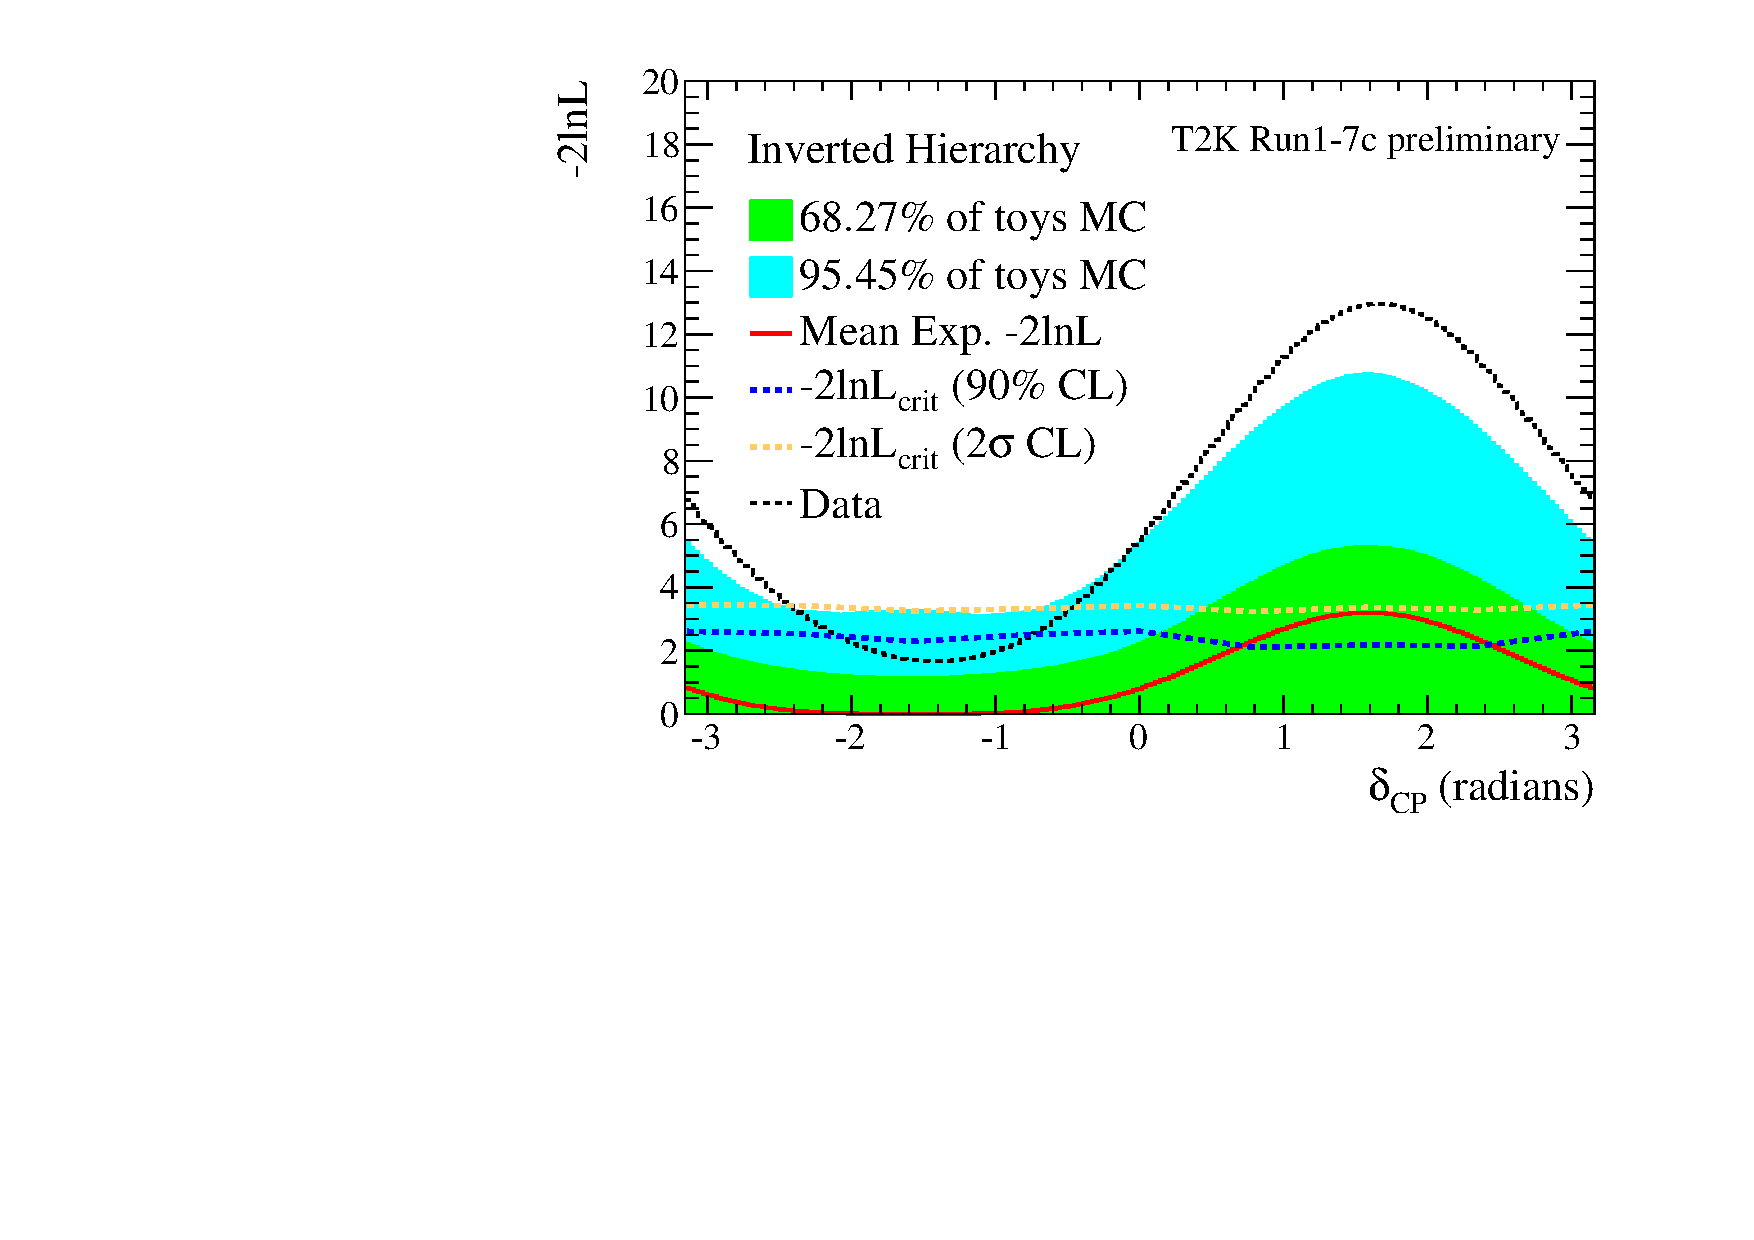
\includegraphics[width=0.9\textwidth]{joint_plots/brazilian_plots/Run17c/brazilian_ih_dcp_mpiover2_trueIH_run17.pdf}
\caption{Inverted hierarchy}
\label{fig:brazilian_mpiover2_trueIH_run17c_ih}
\end{subfigure}
\caption{
The comparison between the expected $<\Delta \chi^2>$ distribution 
for $\delta_{CP} = -\pi/2$ and inverted hierarchy
and the Run 1-7c data set $\Delta \chi^2$ distribution is shown.
10k toy experiments are produced:
all the oscillation parameters which are not parameters of interest
are marginalised using the prior distributions shown in \cref{tab:osc_params_joint_priors}
and applying the reactor constraint.
The red solid line is the expected $<\Delta \chi^2>$ distribution.
The black solid line corresponds to the data $\Delta \chi^2$ distribution.
The green and light blue bands correspond to the regions
that contain respectively 68.27\% and 95.45\% of toy experiments
assuming the $\Delta \chi^2$ p.d.f. to be 1-sided.
The critical values, obtained with the Feldman-Cousins method,
that define the 90\% (blue) and $2\sigma$ (orange) confidence intervals
are shown as well.
}
\label{fig:brazilian_mpiover2_trueIH_run17c}
\end{figure*}

%Since the p-value that shows the consistency of the Run 1-7 $\Delta \chi^2$ 
%with the hypothesis of $\delta_{CP} = -\pi/2$ and inverted hierarchy is 
%low (close to $3 \sigma$) and 10k toy experiments are not enough
%to reach a good precision 
%and more CPU time is needed.
%So the p-value and Z-score as in the previous sections are not shown.
%%However \cref{fig:brazilian_mpiover2_trueIH_run17} is enough to understand the
%%consistency of the Run 1-7 data set $\Delta \chi^2$ distribution
%%with the expected one.

The degeneracy between $\delta_{CP}$ and mass hierarchy can be seen from 
\cref{fig:prob_exclusion_mpiover2_trueIH_run17c} as well, 
where the fraction of toy experiments 
that exclude $\delta_{CP} = 0$ and normal hierarchy is
very similar to the probability to exclude $\delta_{CP} = -\pi/2$ and inverted hierarchy. 

\begin{figure*}[htb]
\center
%
\includegraphics[width=0.9\textwidth]{./images/missing_plot-eps-converted-to.pdf}
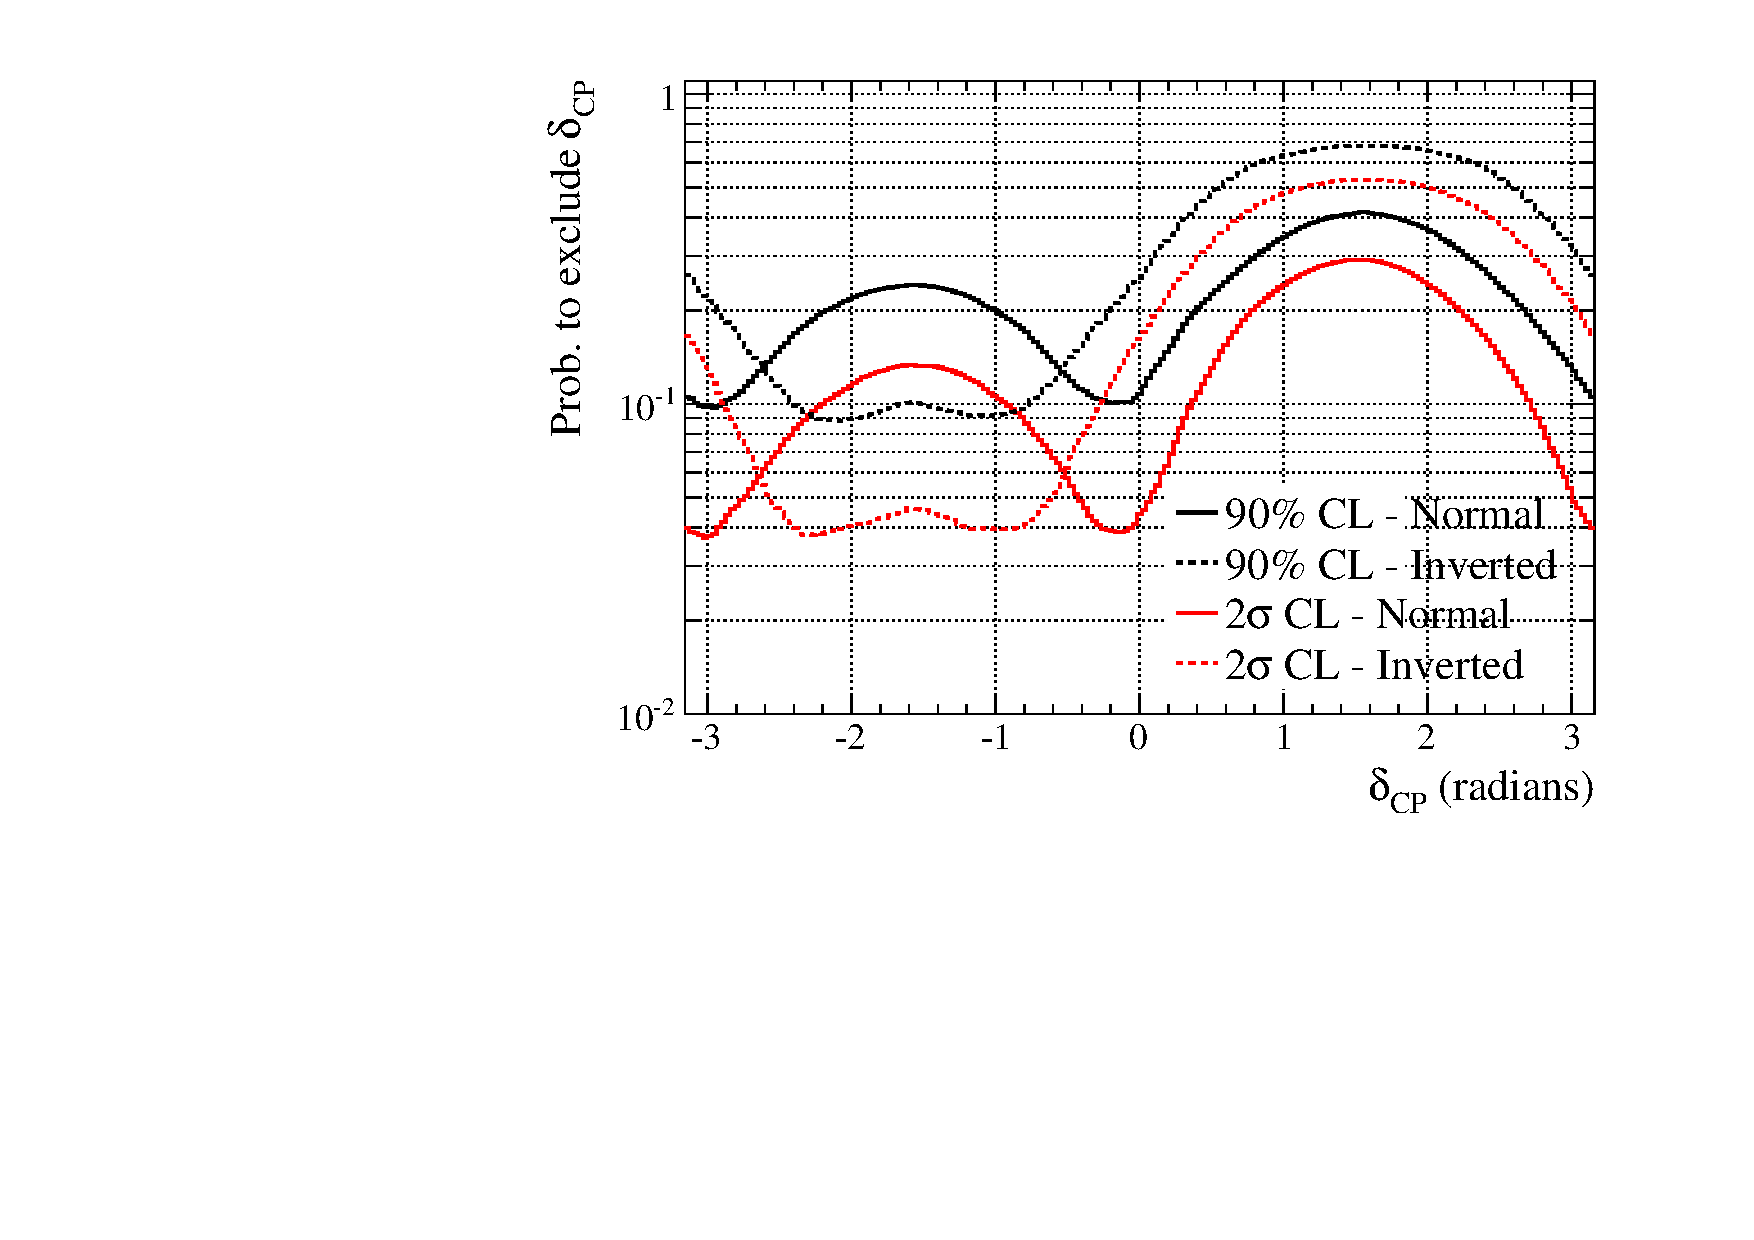
\includegraphics[width=0.49\textwidth]{joint_plots/brazilian_plots/Run17c/prob_excl_dcp_mpiover2_trueIH_run17.pdf}
\caption{
The number of toy experiments that exclude $\delta_{CP}$ at 90\% (black) and $2\sigma$ (red) CL, 
if nature is $\delta_{CP}=-\pi/2$ and inverted hierarchy, is shown
for both normal (solid line) and inverted (dashed line) hierarchy.
}
\label{fig:prob_exclusion_mpiover2_trueIH_run17c}
\end{figure*}



%...........................................................
%
% Discussion about the results
%
%...........................................................

\subsection {Discussion of the Run 1-7c data fit results with sensitivity}
\label{sec:results_discussion_brazilian_run17c}

In \cref{sec:comparison_data_sensi_dcp_run17c} a more detailed analysis of the result is shown.
Though the Run 1-7c data set $\Delta \chi^2$ distribution is consistent with the hypothesis of $\delta_{CP} = -\pi/2$ 
(or $\delta_{CP} = -1.791$) at about $2\sigma$ level.
there is a not negligible probability to exclude $\delta_{CP} = 0$ with a significance of $2\sigma$ 
(more than 9\%), if nature is $\delta_{CP} = -\pi/2$ (or $-1.791$) and normal hierarchy.
In \cref{tab:sensi_fractoys_excluded} the fraction of toy experiments for which 
$\delta_{CP} = 0,\pi$ and normal and inverted hierarchy are excluded at 90\% and $2\sigma$ CL. 
The conclusions are very similar to Run 1-7c,
though the tension between data and expectation is now slightly reduced
and always within $2 \sigma$.

\begin{table}[htb]
\centering
\begin{tabular}{| c | c || c | c | c |}
\hline
\multicolumn{4}{| c |}{\textcolor{blue}{True: $\delta_{CP} = -\pi/2$ - normal hierarchy}}  \\
\hline
\bf $\delta_{CP}$	& hierarchy	& 90\% CL       	& $2\sigma$ CL  \\ \hline
\hline
 $0$ 				& normal		& 0.196           	& 0.092	\\ \hline
 $\pi$ 			& normal		& 0.173           	& 0.070 	\\ \hline
 $0$ 				& inverted		& 0.470           	& 0.355 	\\ \hline
 $\pi$ 			& inverted		& 0.471        	& 0.359 	\\ \hline
\hline
\multicolumn{4}{| c |}{\textcolor{blue}{True: $\delta_{CP} = -1.791$ - normal hierarchy}}  \\
\hline
$\delta_{CP}$		& hierarchy	& 90\% CL       	& $2\sigma$ CL  \\ \hline
\hline
 $0$ 				& normal		& 0.191           	& 0.085  	\\ \hline
 $\pi$ 			& normal		& 0.157             & 0.065	\\ \hline
 $0$ 				& inverted		& 0.453             & 0.339 	\\ \hline
 $\pi$ 			& inverted		& 0.465             & 0.345	\\ \hline
\hline
\multicolumn{4}{| c |}{\textcolor{blue}{True: $\delta_{CP} = 0$ - normal hierarchy}}  \\
\hline
$\delta_{CP}$		& hierarchy	& 90\% CL       	& $2\sigma$ CL  \\ \hline
\hline
 $0$ 				& normal		& 0.108    		& 0.048	\\ \hline
 $\pi$ 			& normal		& 0.149      	& 0.067 	\\ \hline
 $0$ 				& inverted		& 0.208	    	& 0.123 	\\ \hline
 $\pi$ 			& inverted		& 0.177	       	& 0.109	\\ \hline
\hline
\multicolumn{4}{| c |}{\textcolor{blue}{True: $\delta_{CP} = -\pi/2$ - inverted hierarchy}}  \\
\hline
$\delta_{CP}$		& hierarchy	& 90\% CL       	& $2\sigma$ CL  \\ \hline
\hline
 $0$ 				& normal		& 0.108           	& 0.044	\\ \hline
 $\pi$ 			& normal		& 0.106             & 0.040 	\\ \hline
 $0$ 				& inverted		& 0.255             & 0.162	\\ \hline
 $\pi$ 			& inverted		& 0.261             & 0.166	\\ \hline
\end{tabular}
\caption{
The fraction of toy experiments for which $\delta_{CP} = 0,\pi$ and normal and inverted hierarchy
are excluded at 90\% and $2\sigma$ CL is shown for different true values of $\delta_{CP}$ and mass hierarchy.
10k toy experiments are used. 
}
\label{tab:sensi_fractoys_excluded}
\end{table}


\clearpage









